\chapter{Ergebnisse}
In diesem Abschnitt werden exemplarisch für zwei Eingangs-Phasenrauschleistungsspektren Simulationsergebnisse aus MRiLab vorgestellt und bewertet.

\section{Gewählte Simulationsparameter}
Die MRiLab-Simulationsparameter werden so gewählt, dass sie einem realen Bruker BioSpec Tomographen möglichst gut entsprechen (vgl. \autoref{tab:brukerMRIparam}). Einige Parameter, wie die Auflösungen müssen jedoch verkleinert werden, da größere Werte zu unvorhersehbaren Abstürzen von MRiLab führen. Die Größe des Aufnahmefelds (FOV) wird den Abmessungen des Phantoms angepasst. Die gewählten Parameter sind in \autoref{tab:mrilabparamSim} zusammengefasst.

\begin{table}[H]
	\centering
	\caption[gewählte Simulationsparameter]{Für diesen Abschnitt gewählte Simulationsparameter}
	\label{tab:mrilabparamSim}
	\begin{tabularx}{0.5\textwidth}{lX}
		\toprule
		\textbf{Parameter} & \textbf{Werte}\\
		\midrule
		FOVFreq    & \SI{80}{\mm}\\
		FOVPhase   & \SI{80}{\mm}\\
		ResFreq    & 160\\
		ResPhase   & 160\\
		SliceThick & \SI{2}{\mm}\\
		B0         & \SI{15}{\tesla} \\
		\bottomrule
		\end{tabularx}
		\end{table}

\section{Referenz-Schnittbild}
Zum visuellen Vergleich und für die Nutzung der Bildqualitätsmetriken SSIM und MSE ist ein Referenzbild notwendig. Dazu wird eine Simulation mit einer Spinecho-Sequenz ohne Rauschen durchgeführt (siehe \autoref{fig:R}).

\begin{figure}[H]
	\centering
	\resizebox{!}{!}{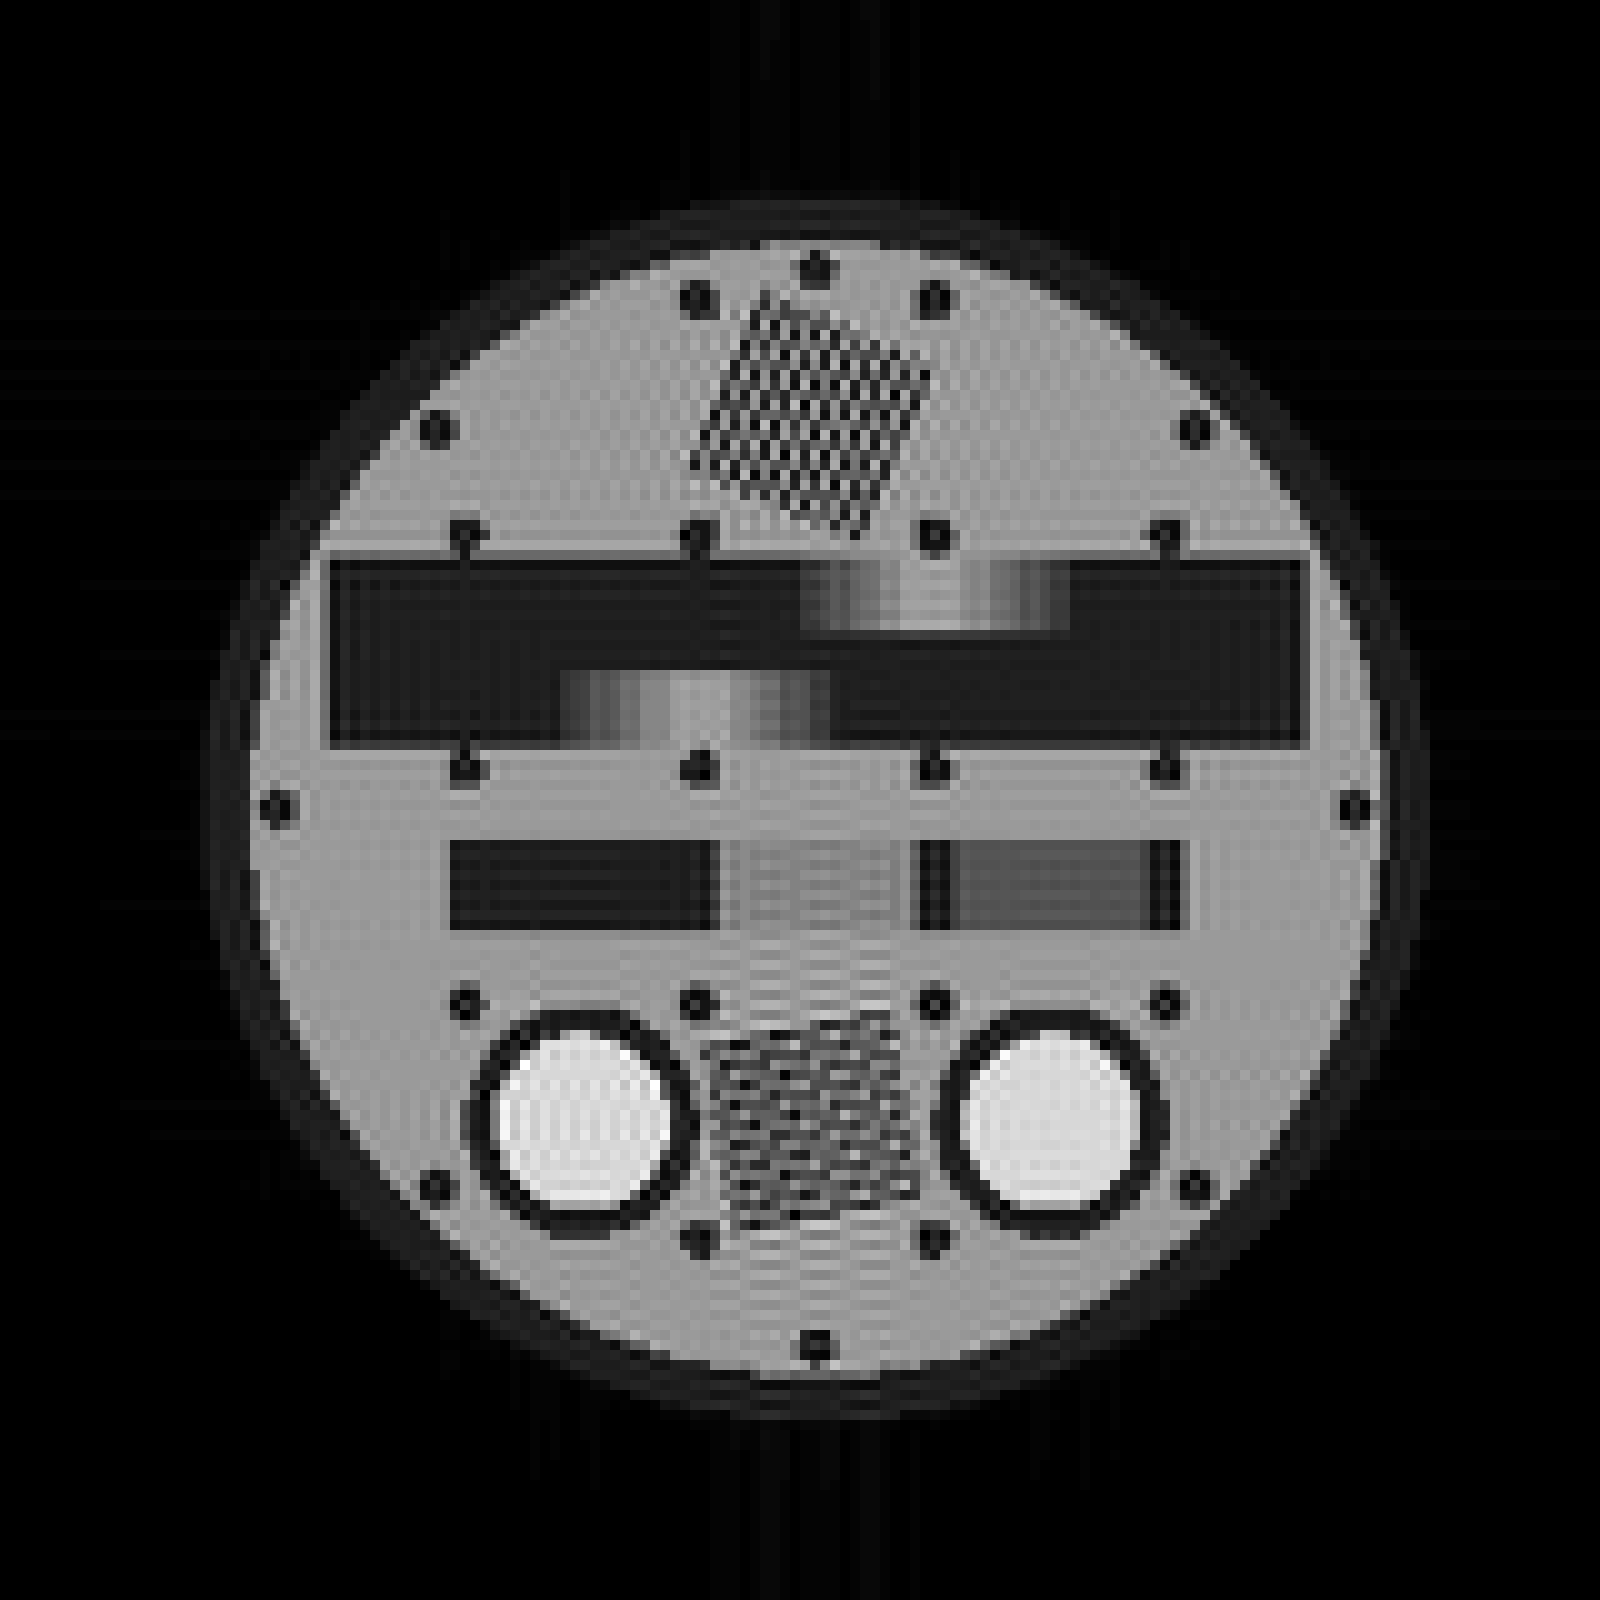
\includegraphics[width=0.47\textwidth]{img/results/Series13_REF_OUT.png}}
	\caption[Referenzbild]{Referenzbild $R[i,j]$}
	\label{fig:R}
\end{figure}

In den weiteren Unterabschnitten sind jeweils, zusätzlich zu den simulierten Schnittbildern, Differenzbilder abgebildet. Diese geben, in Falschfarben kodiert, die Abweichungen vom Referenzbild an. Das Differenzbild $D[i,j]$ berechnet sich dabei aus dem Referenzbild $R[i,j]$ und dem jeweils betrachteten Schnittbild $X[i,j]$ nach
\begin{equation}
	D[i,j]=\left| X[i,j]-R[i,j]\right|.
\end{equation}

Durch die Verwendung der Falschfarben-Darstellung mit der MATLAB-Farbpalette \texttt{Jet} (\autoref{fig:colorJet}) werden kleine Unterschiede deutlicher sichtbar, als bei einer Graustufen-Palette. Die simulierten Schnittbilder werden, wie in der MRT üblich, als Graustufenbilder dargestellt.
\begin{figure}[H]
	\centering
	\resizebox{!}{!}{\includegraphics[]{img/jetColormap.tikz}}
	\caption[]{Farbpalette \texttt{Jet} in MATLAB}
	\label{fig:colorJet}
\end{figure}


\section{LMK04821}

\subsection{Spinecho-Sequenz}

\begin{figure}[H]
	\centering
	\subcaptionbox{Rekonstruiertes Schnittbild}{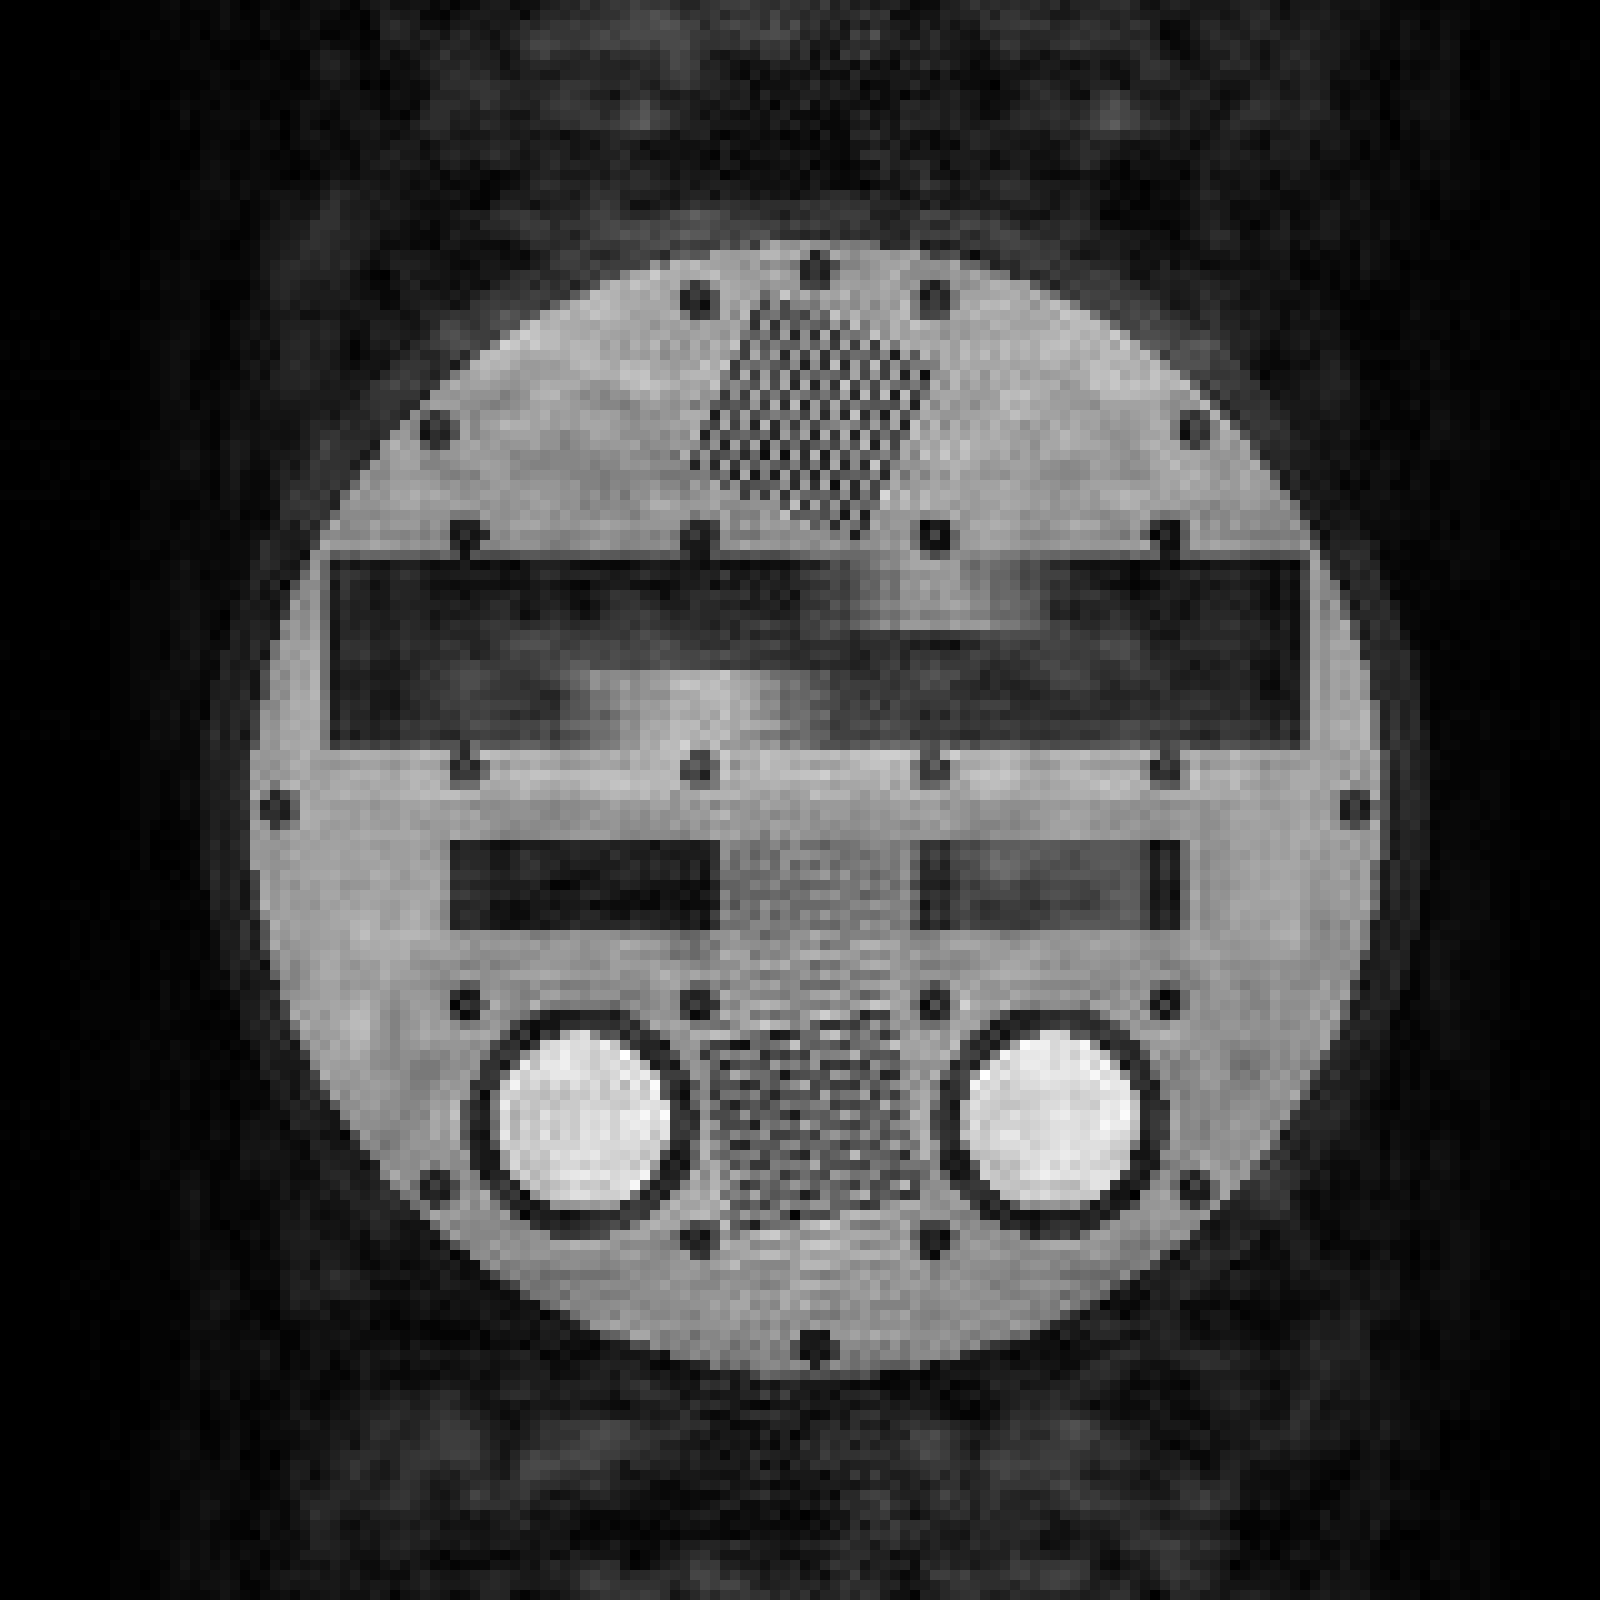
\includegraphics[width=0.47\textwidth]{img/results/lmk/SE/Series15_OUT.png}}
	\hfill
	\subcaptionbox{Differenzbild $D[i,j]$}{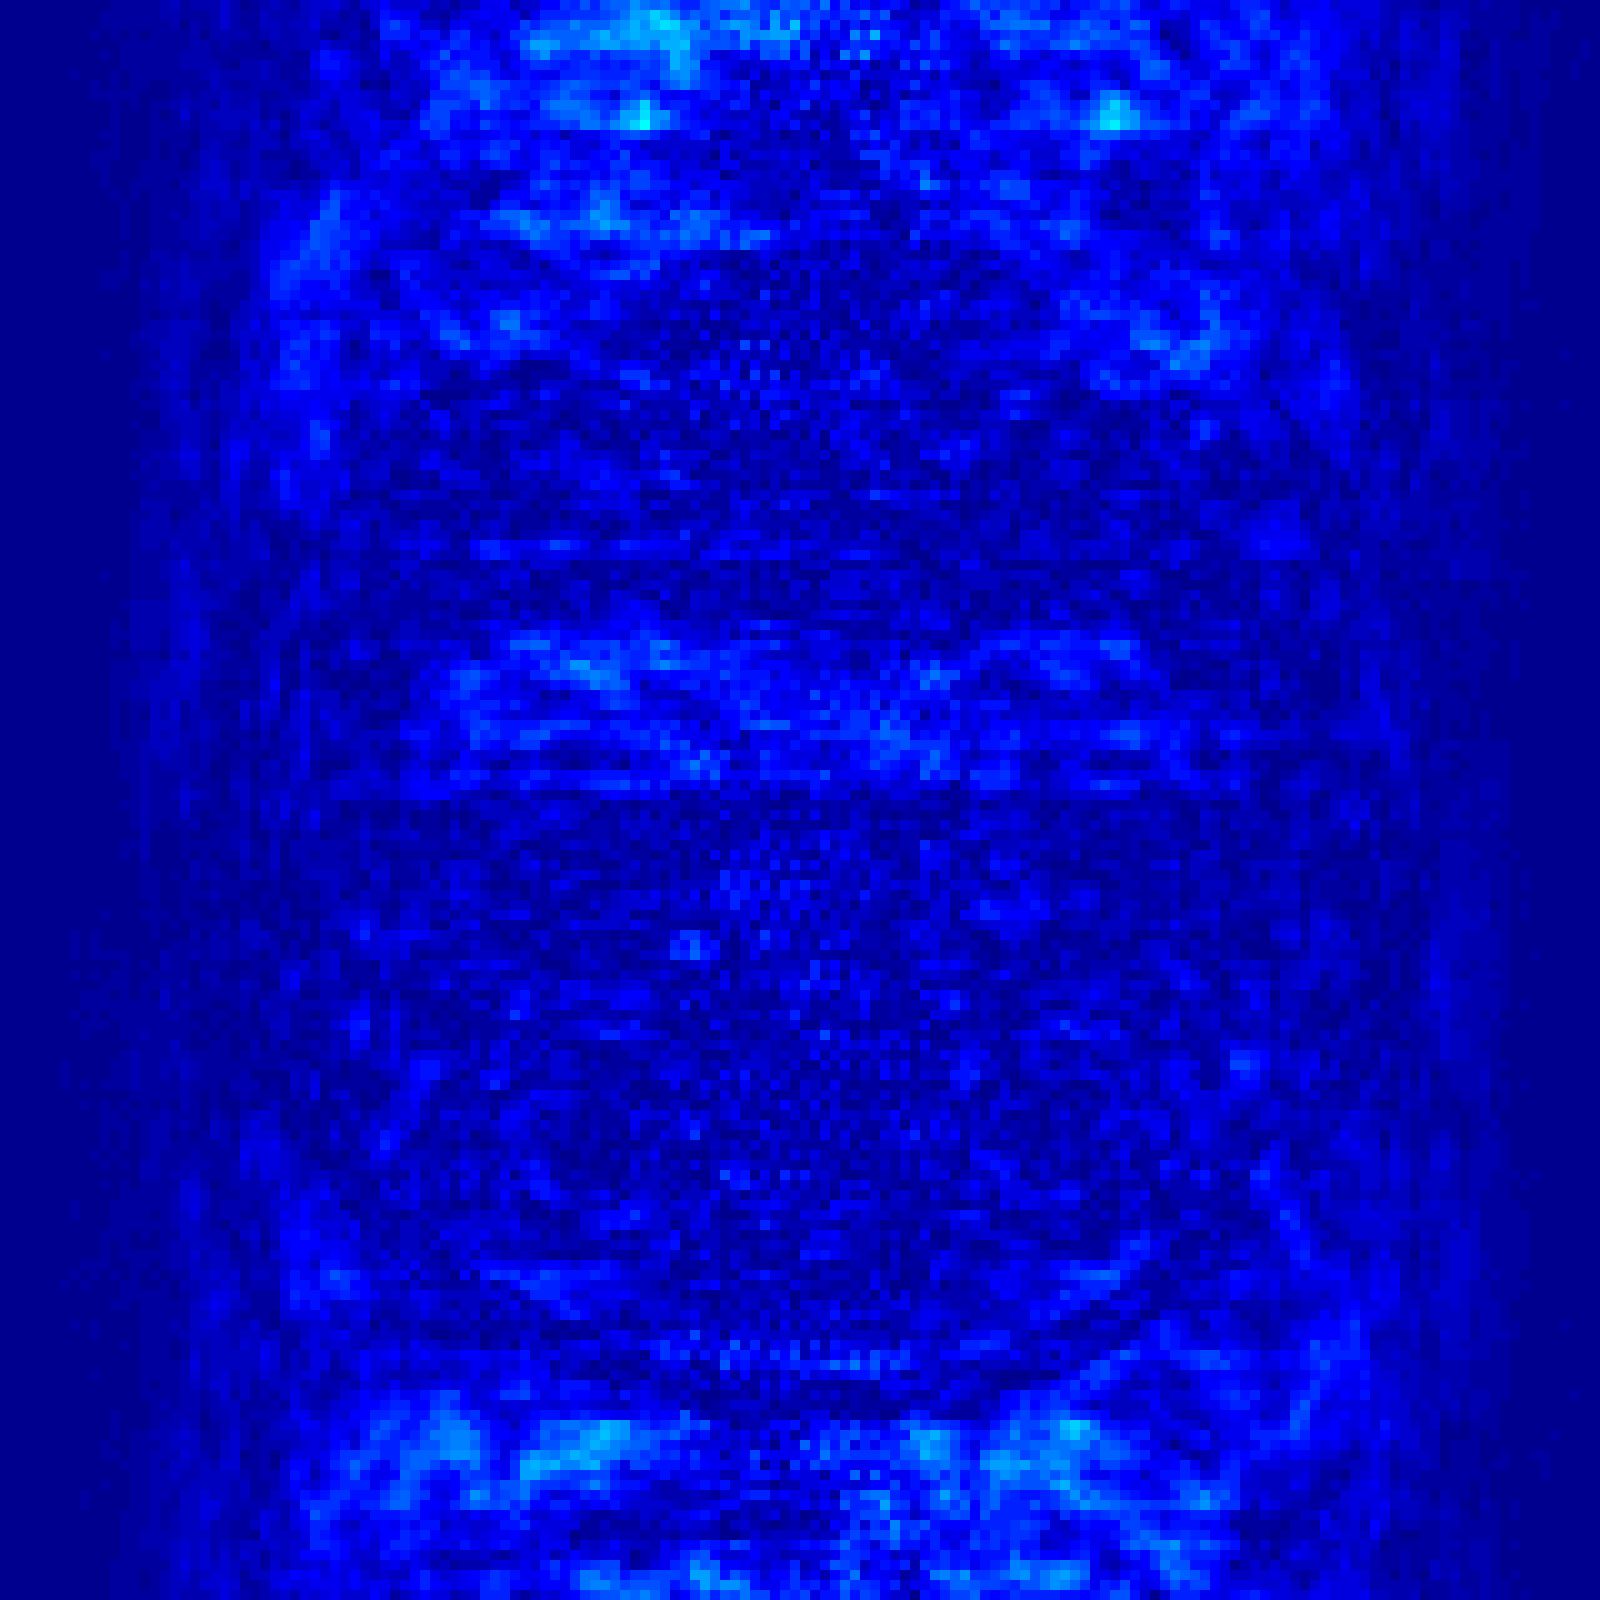
\includegraphics[width=0.47\textwidth]{img/results/lmk/SE/Series15_DIFF.png}}
	\caption[LMK04821 in MR-Tomograph mit aktivem Gradientensystem (SE) (1)]{Simulationsergebnis LMK04821 in MR-Tomograph mit aktivem Gradientensystem (Spinecho-Sequenz); $MSE=0.0057$, $SSIM=0.6111$}
	\label{fig:resLMKse1}	
\end{figure}

\begin{figure}[H]
	\centering
	\subcaptionbox{Rekonstruiertes Schnittbild}{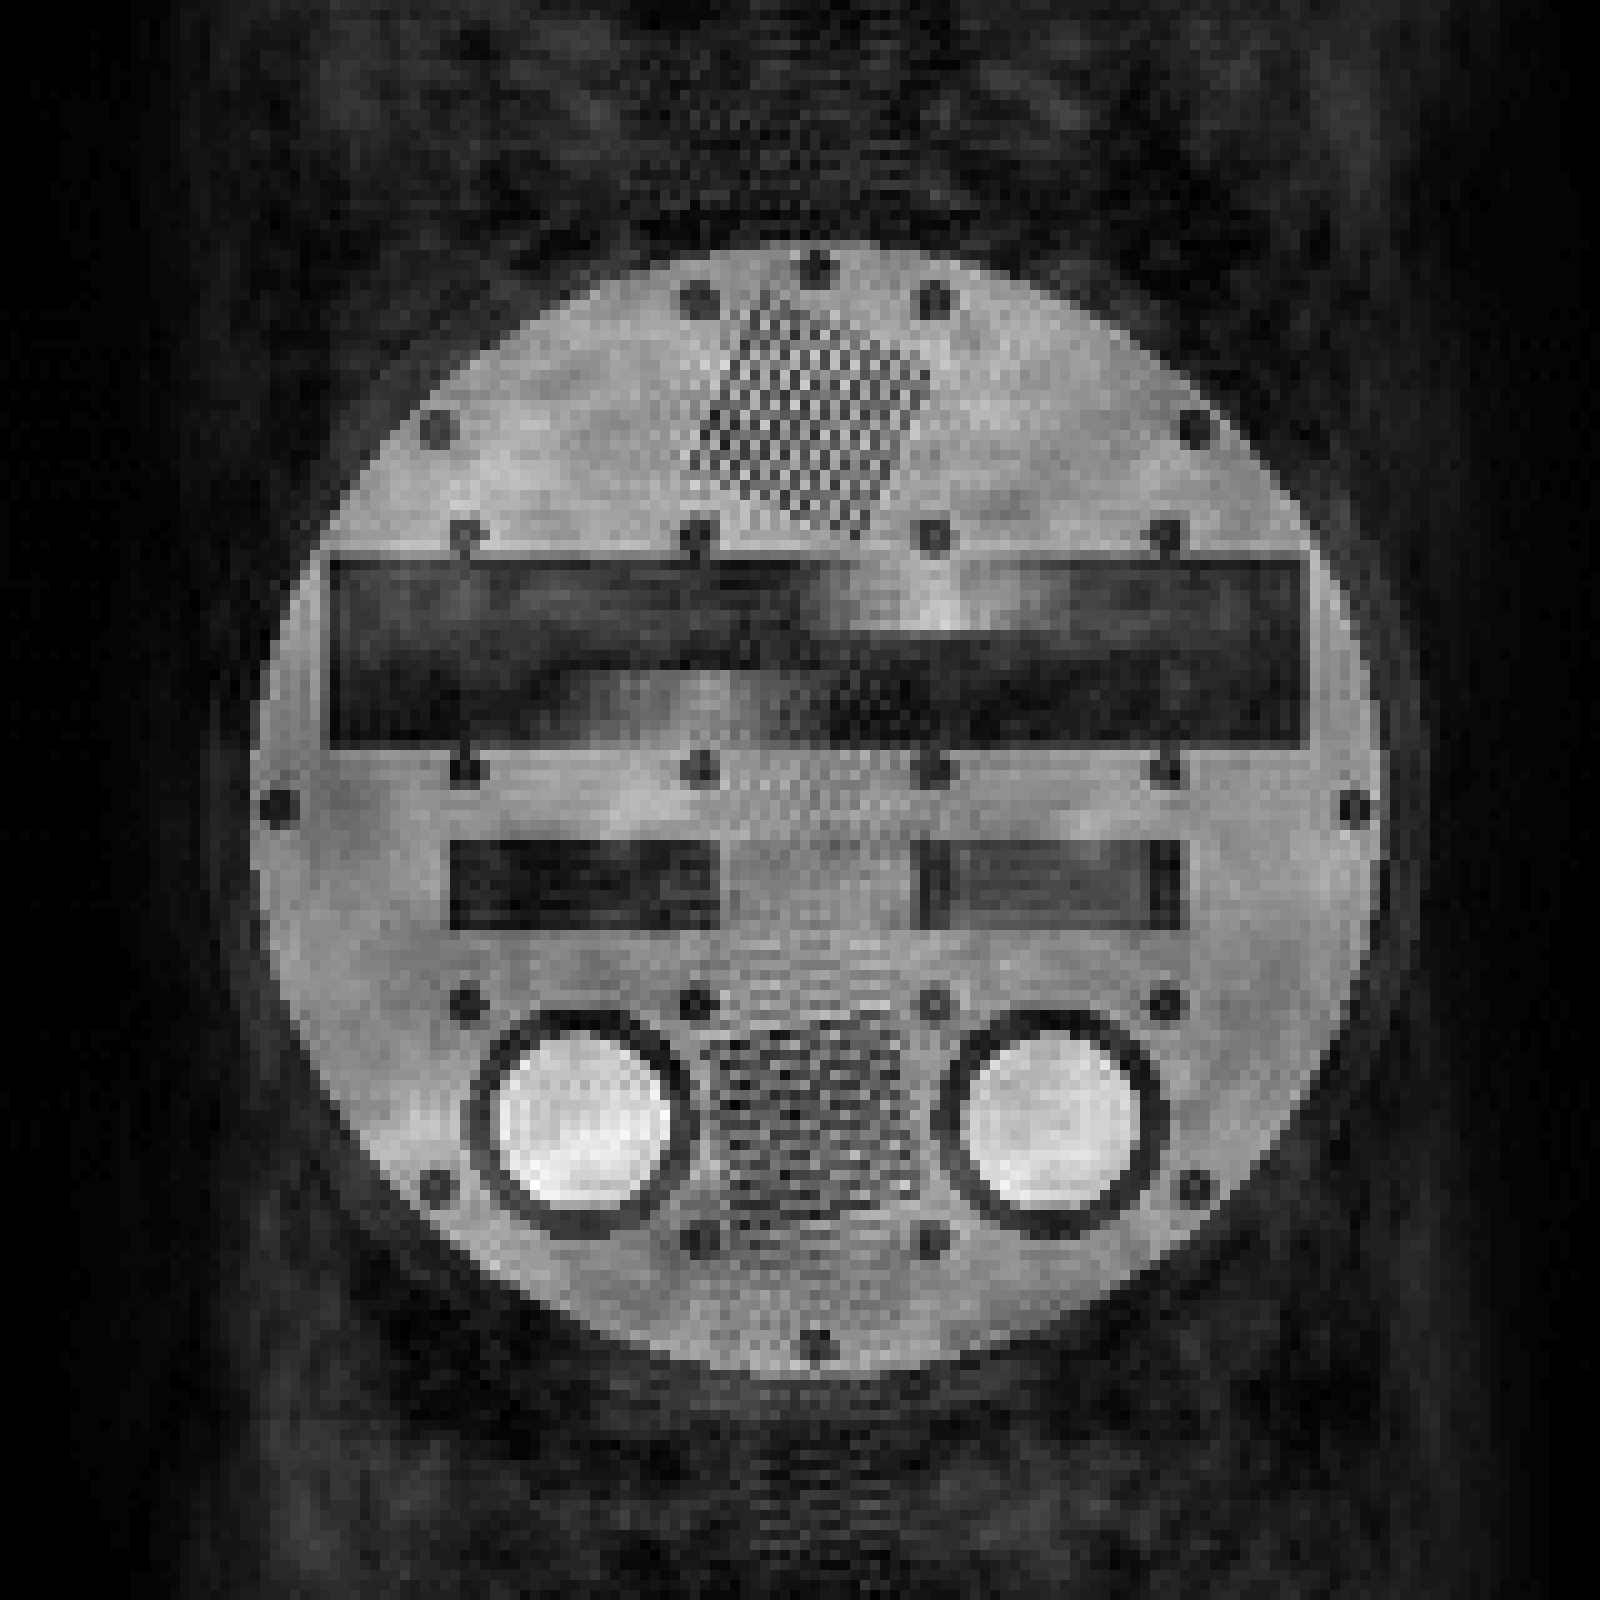
\includegraphics[width=0.47\textwidth]{img/results/lmk/SE/Series16_OUT.png}}
	\hfill
	\subcaptionbox{Differenzbild $D[i,j]$}{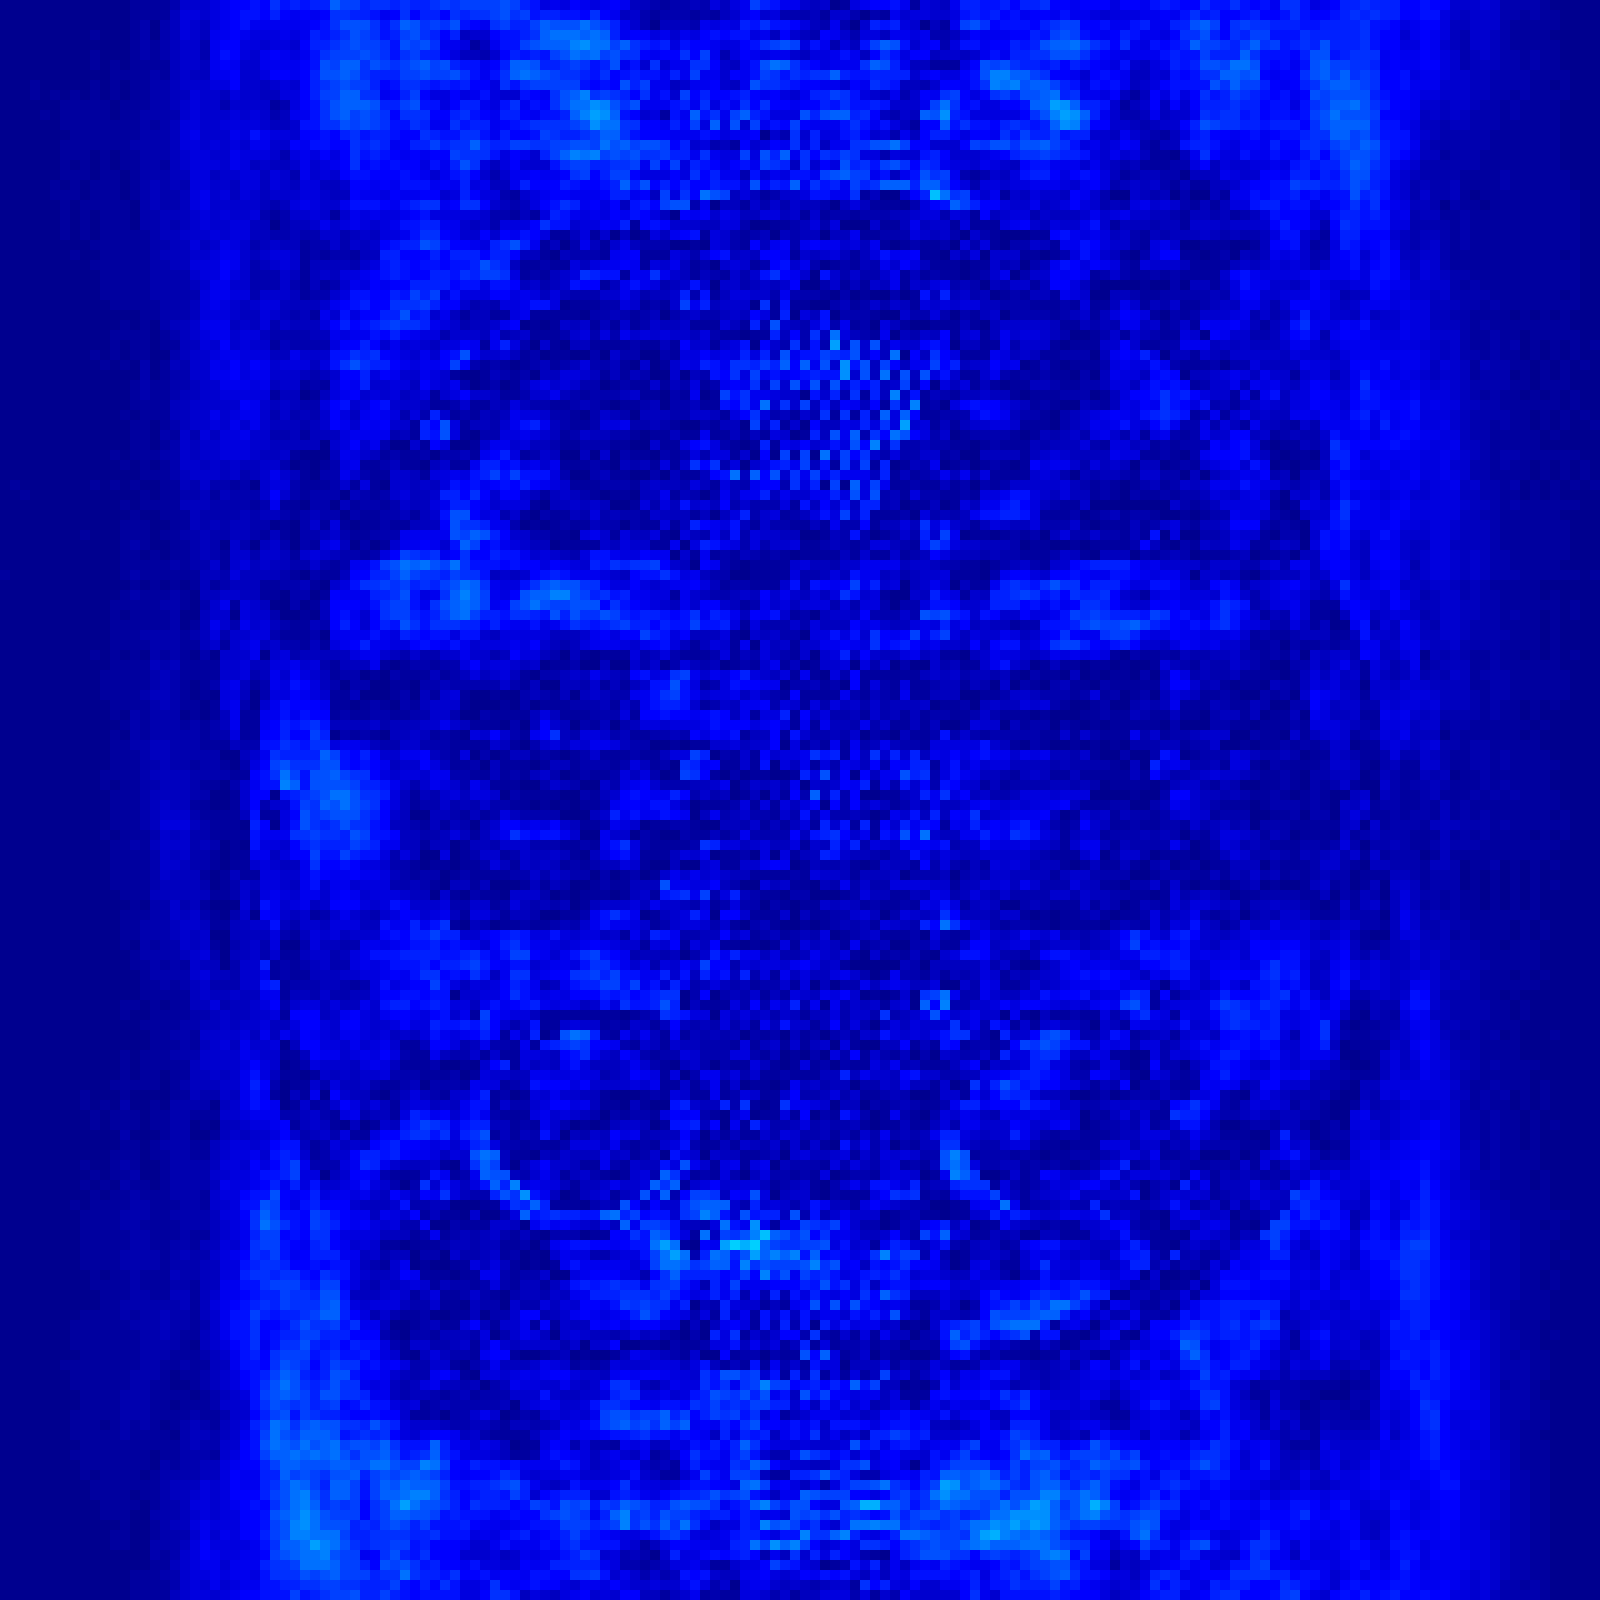
\includegraphics[width=0.47\textwidth]{img/results/lmk/SE/Series16_DIFF.png}}
	\caption[LMK04821 in MR-Tomograph mit aktivem Gradientensystem (SE) (2)]{Simulationsergebnis LMK04821 in MR-Tomograph mit aktivem Gradientensystem (Spinecho-Sequenz); $MSE=0.0074$, $SSIM=0.5616$}
	\label{fig:resLMKse2}	
\end{figure}

\begin{figure}[H]
	\centering
	\subcaptionbox{Rekonstruiertes Schnittbild}{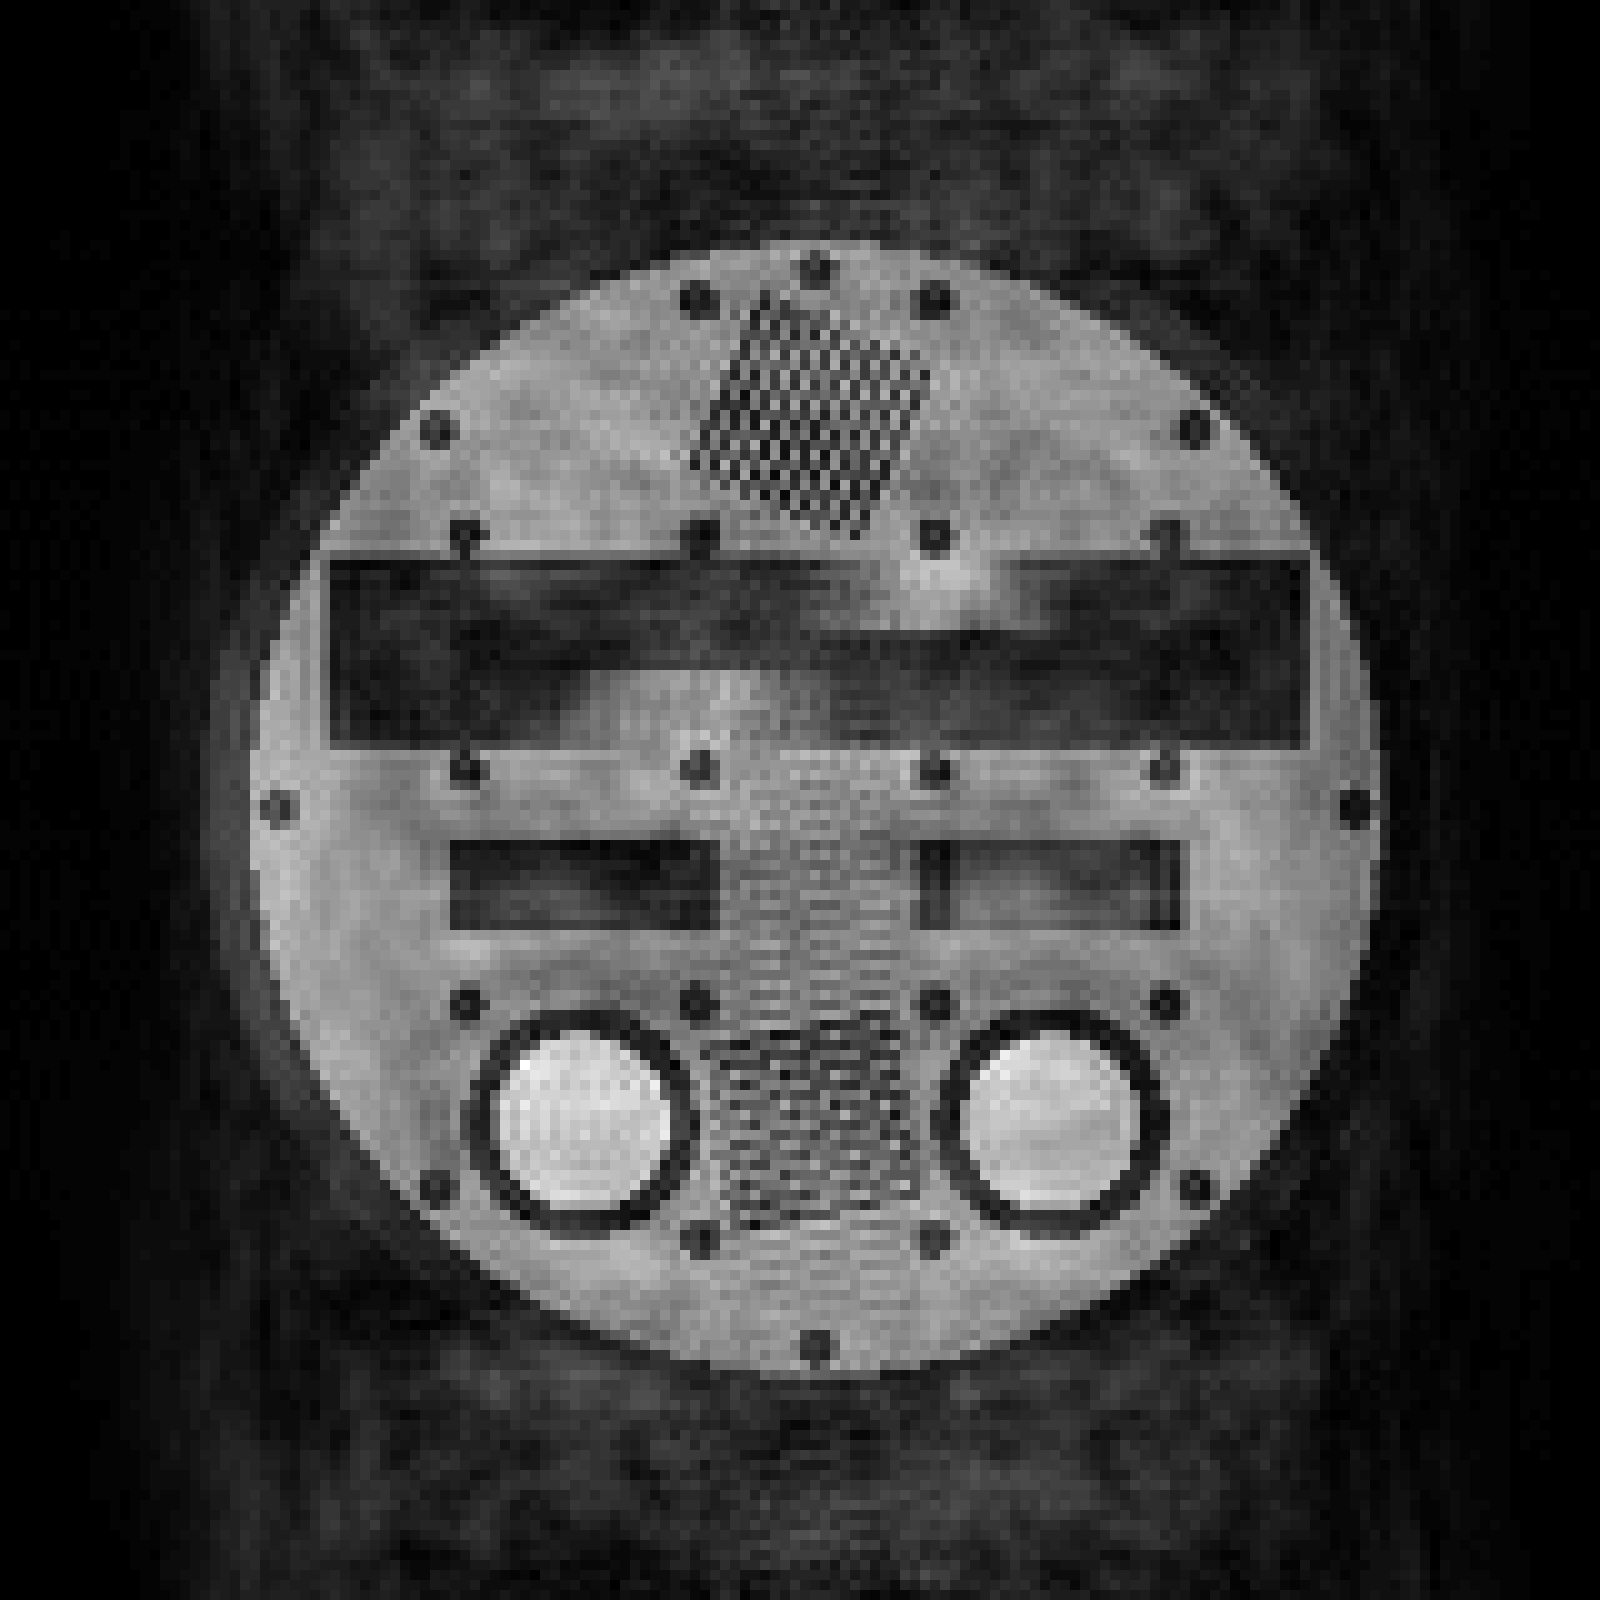
\includegraphics[width=0.47\textwidth]{img/results/lmk/SE/Series17_OUT.png}}
	\hfill
	\subcaptionbox{Differenzbild $D[i,j]$}{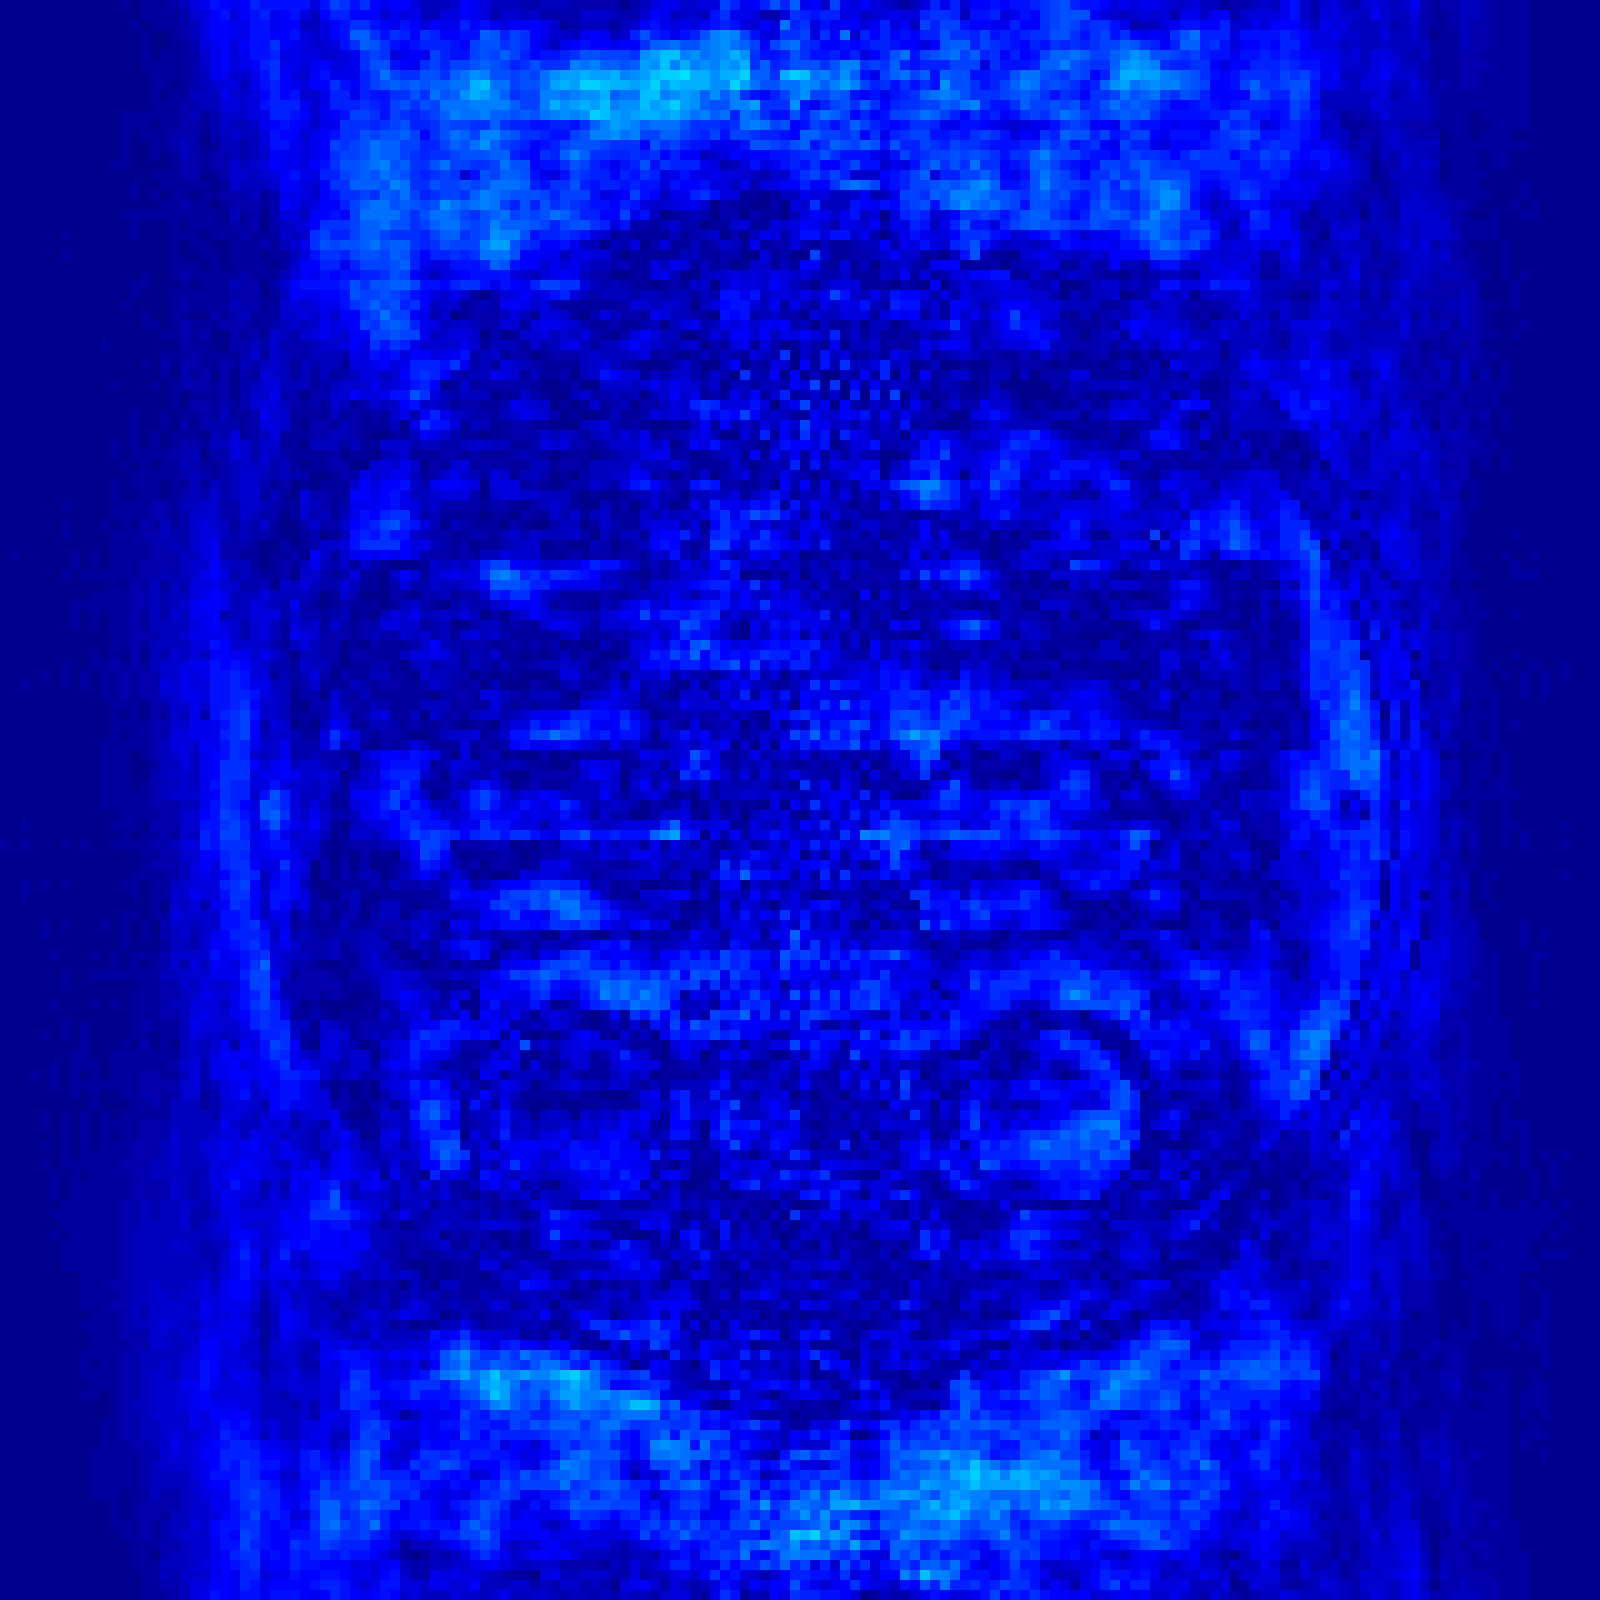
\includegraphics[width=0.47\textwidth]{img/results/lmk/SE/Series17_DIFF.png}}
	\caption[LMK04821 in MR-Tomograph mit aktivem Gradientensystem (SE) (3)]{Simulationsergebnis LMK04821 in MR-Tomograph mit aktivem Gradientensystem (Spinecho-Sequenz); $MSE=0.0086$, $SSIM=0.5813$}
	\label{fig:resLMKse3}	
\end{figure}

\subsection{EPI-Sequenz}

\begin{figure}[H]
	\centering
	\subcaptionbox{Rekonstruiertes Schnittbild}{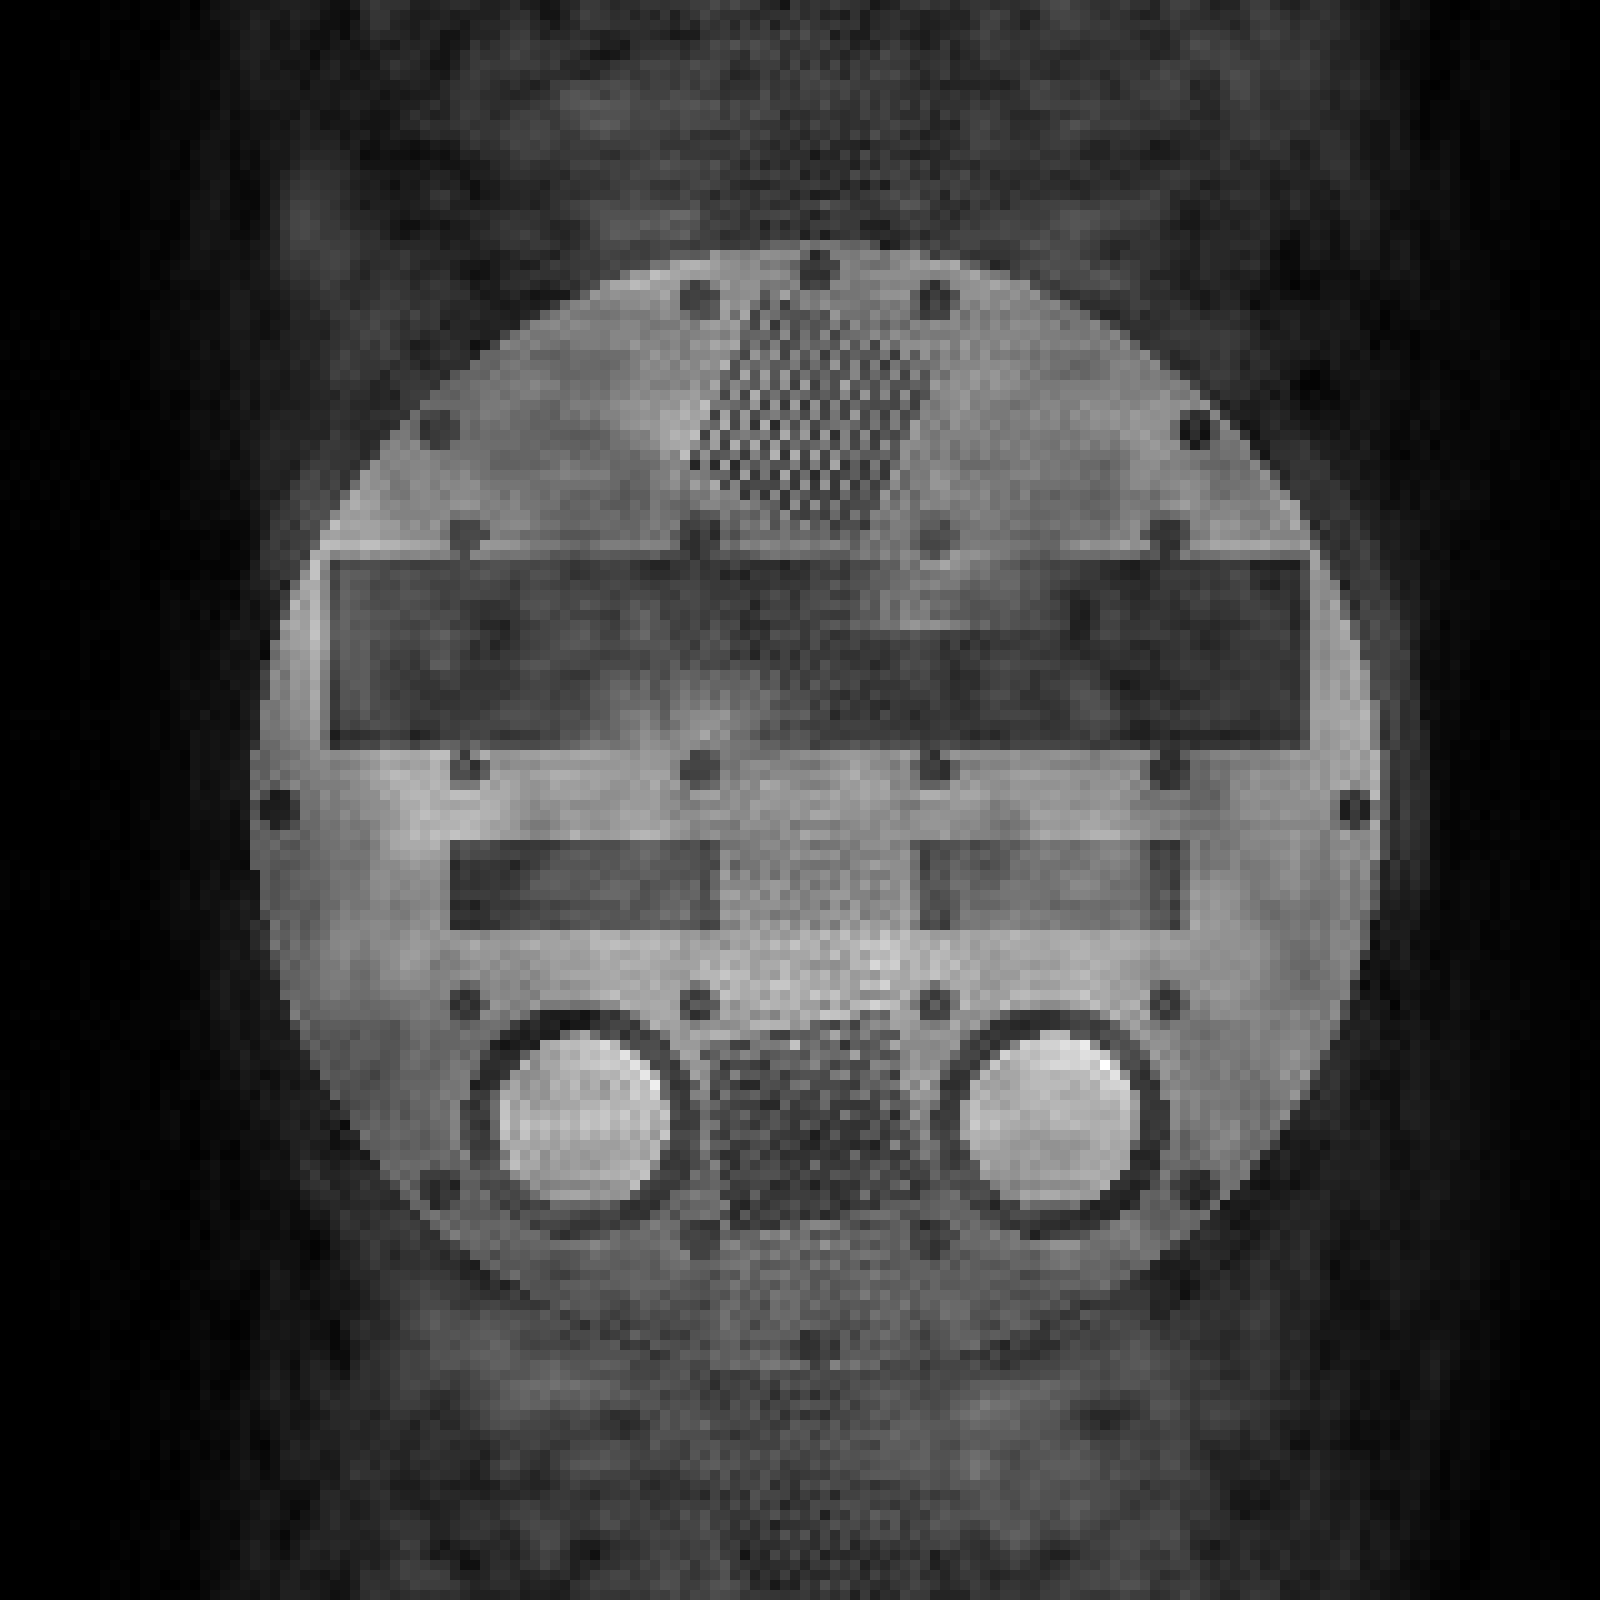
\includegraphics[width=0.47\textwidth]{img/results/lmk/EPI/Series18_OUT.png}}
	\
	\subcaptionbox{Differenzbild $D[i,j]$}{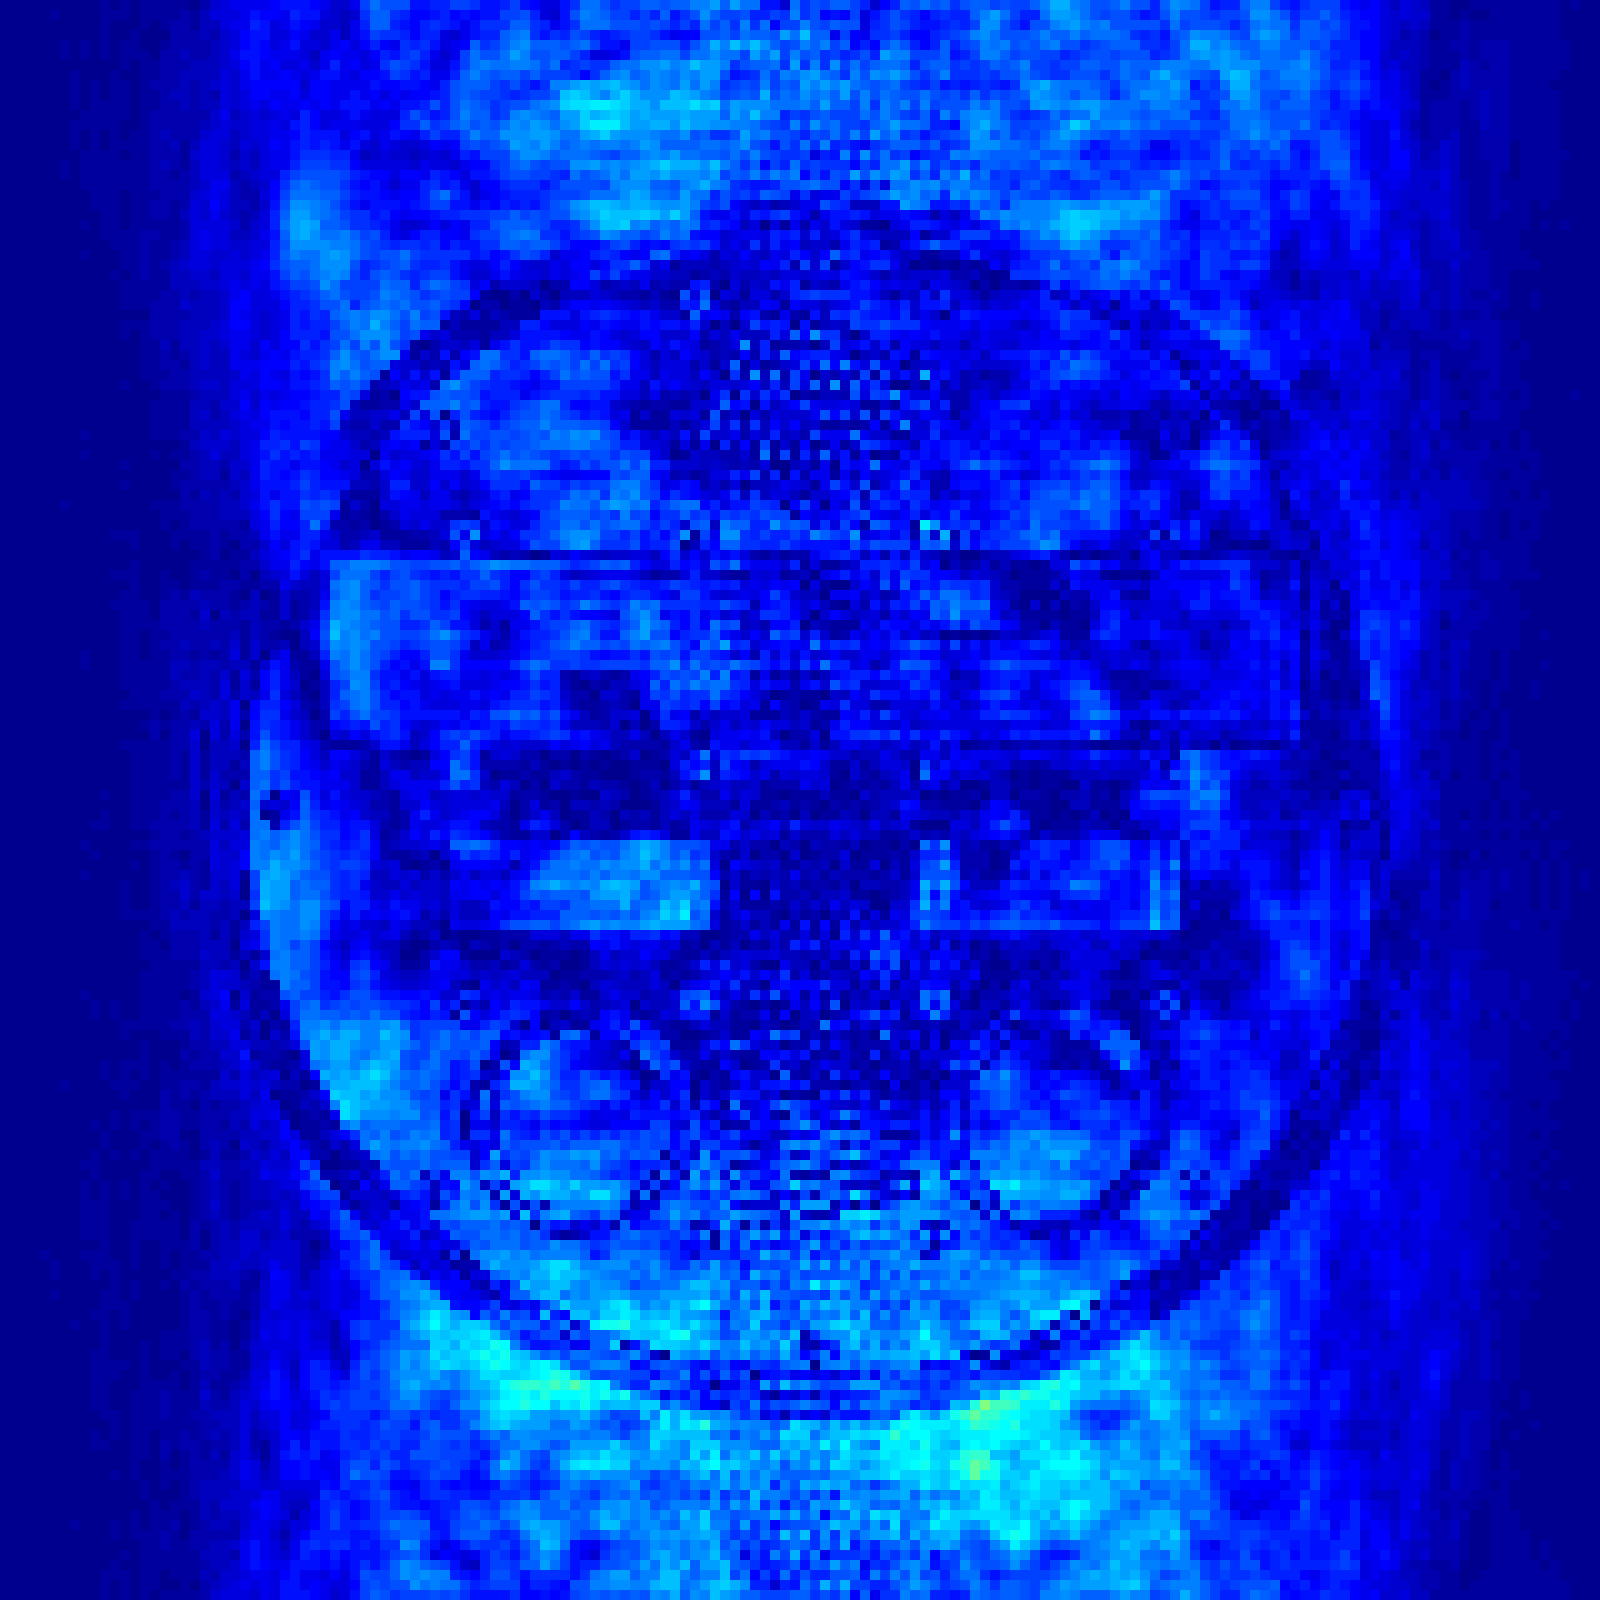
\includegraphics[width=0.47\textwidth]{img/results/lmk/EPI/Series18_DIFF.png}}
	\caption[LMK04821 in MR-Tomograph mit aktivem Gradientensystem (EPI) (1)]{Simulationsergebnis LMK04821 in MR-Tomograph mit aktivem Gradientensystem (EPI-Sequenz); $MSE=0.0188$, $SSIM=0.5289$}
	\label{fig:resLMKepi1}	
\end{figure}

\begin{figure}[H]
	\centering
	\subcaptionbox{Rekonstruiertes Schnittbild}{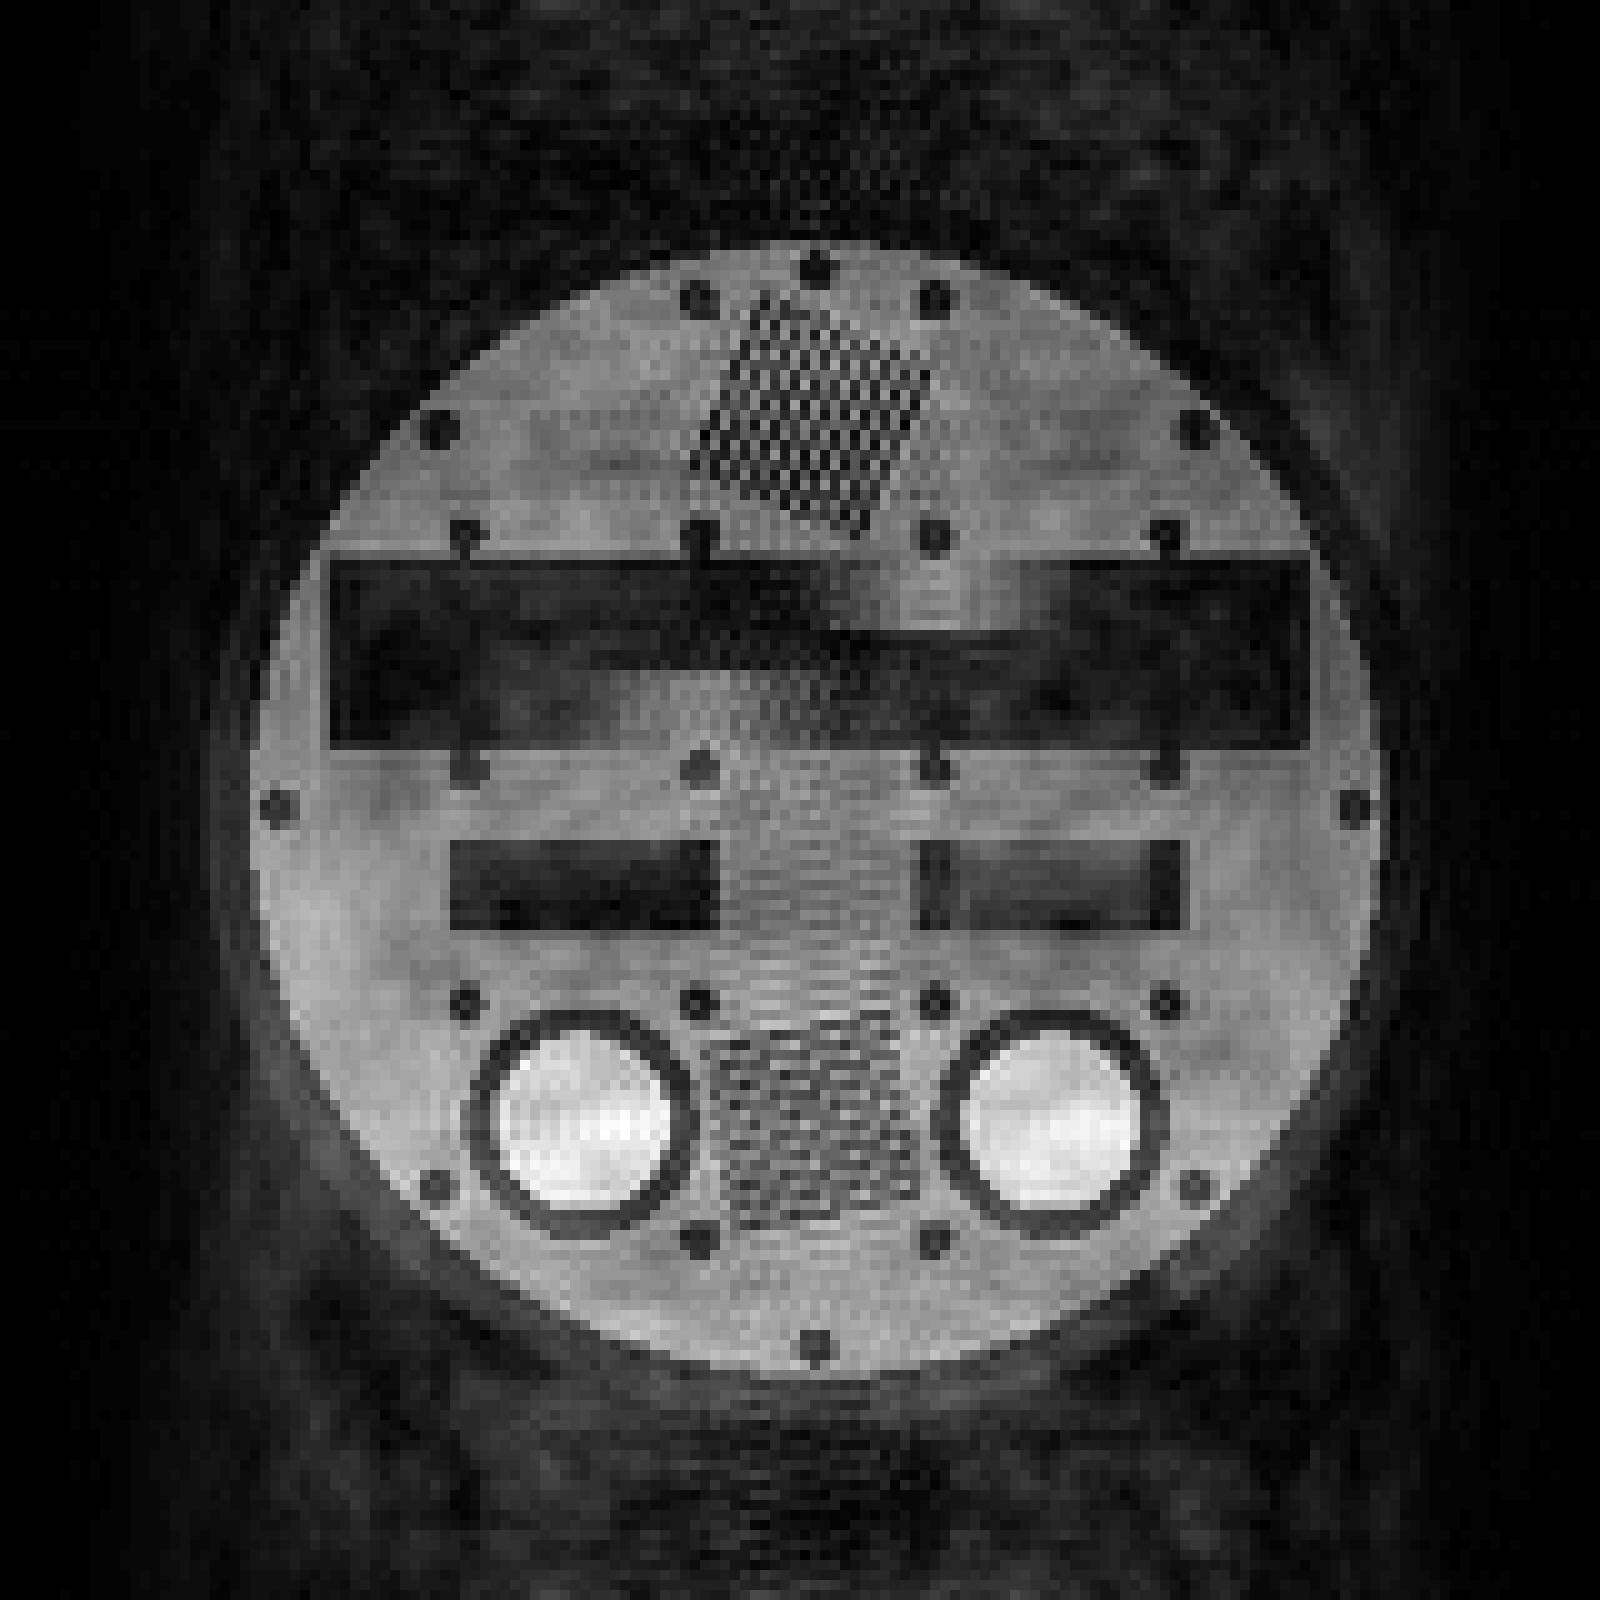
\includegraphics[width=0.47\textwidth]{img/results/lmk/EPI/Series19_OUT.png}}
	\
	\subcaptionbox{Differenzbild $D[i,j]$}{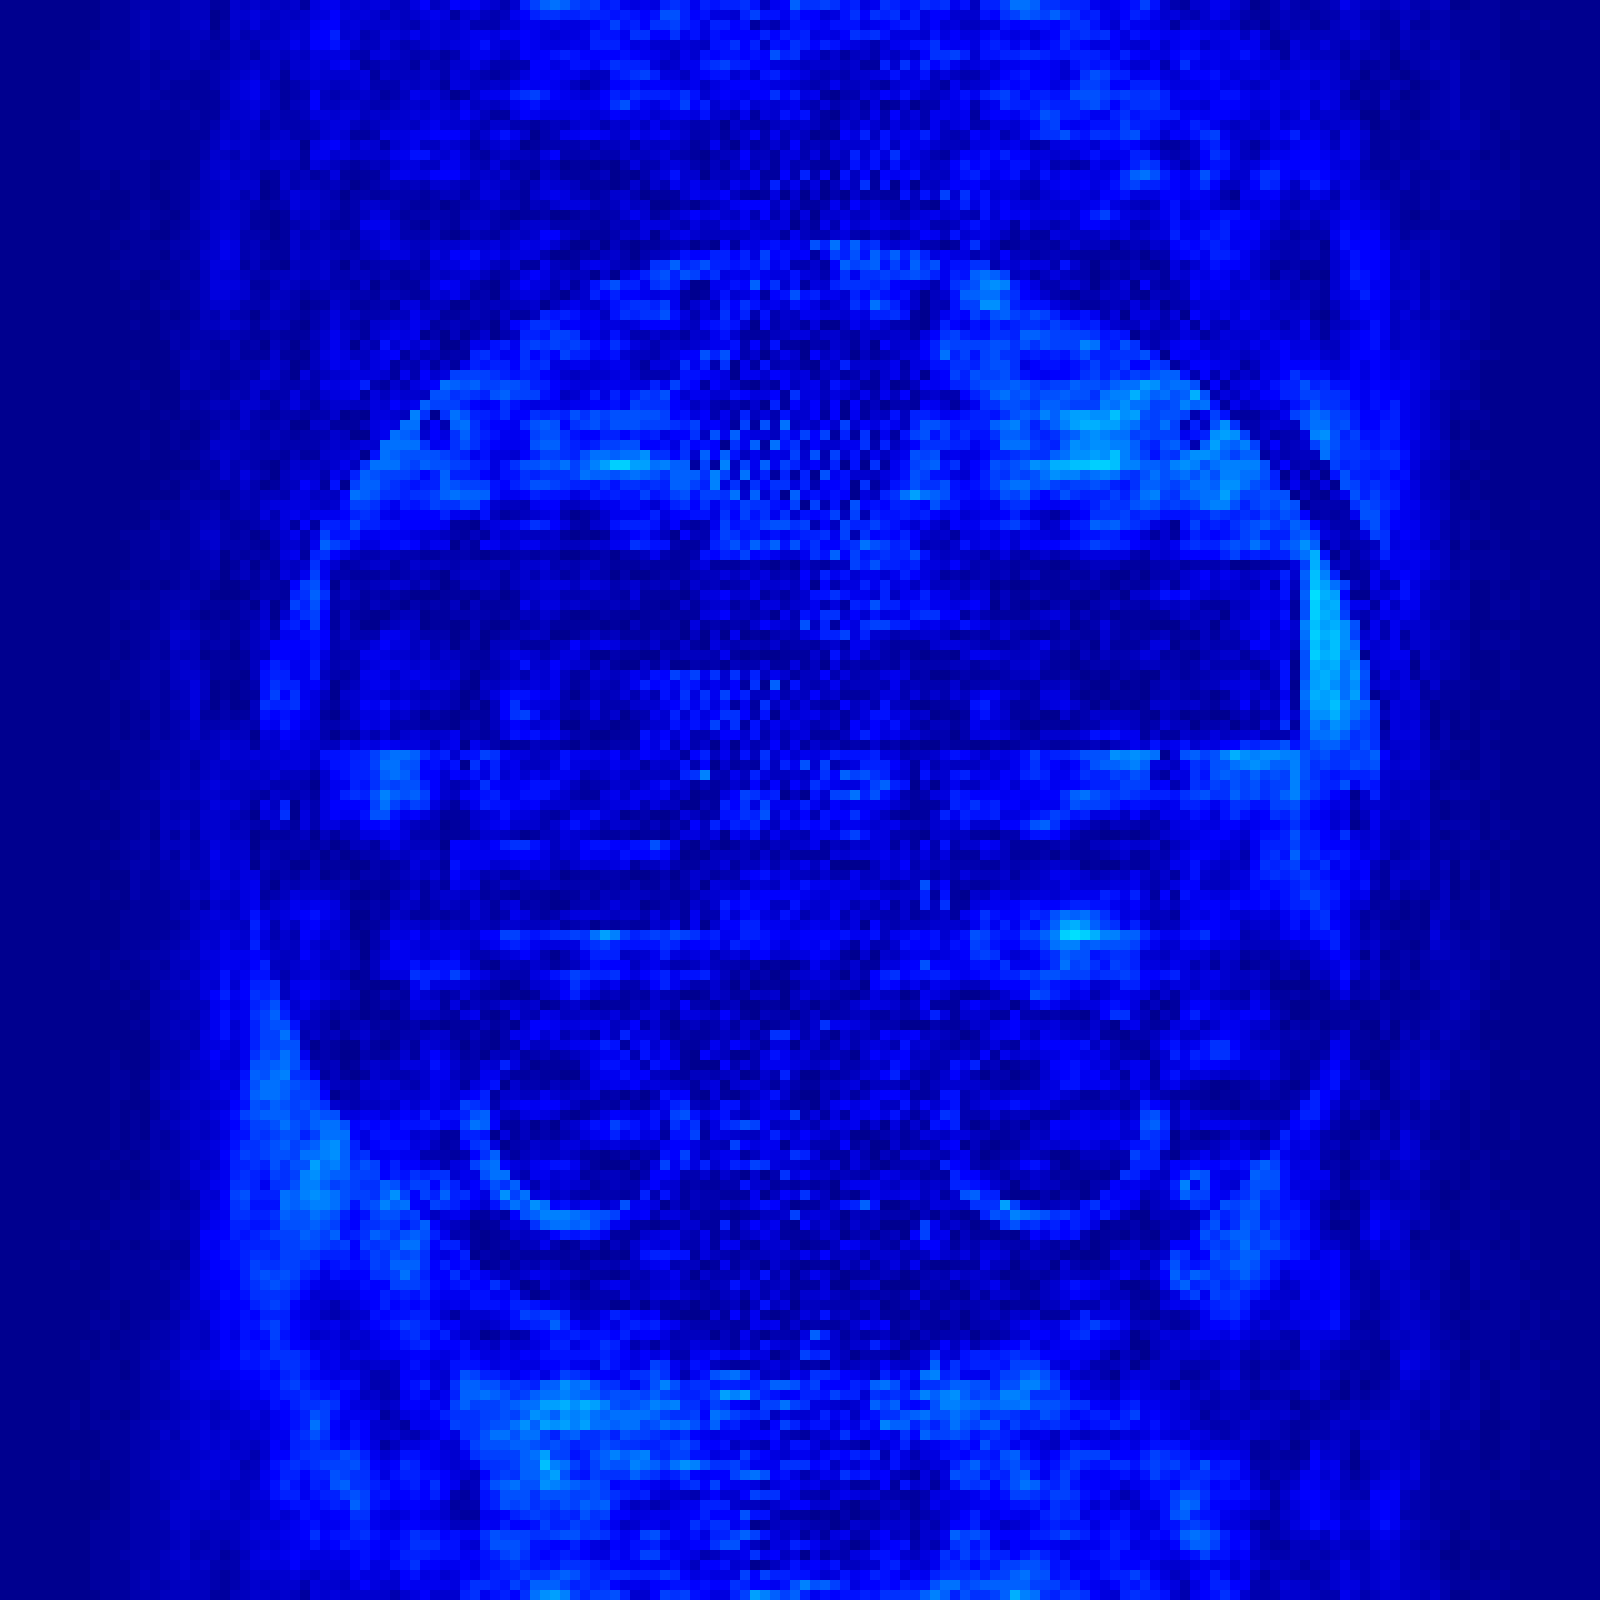
\includegraphics[width=0.47\textwidth]{img/results/lmk/EPI/Series19_DIFF.png}}
	\caption[LMK04821 in MR-Tomograph mit aktivem Gradientensystem (EPI) (2)]{Simulationsergebnis LMK04821 in MR-Tomograph mit aktivem Gradientensystem (EPI-Sequenz); $MSE=0.0082$, $SSIM=0.5883$}
	\label{fig:resLMKepi2}	
\end{figure}

\begin{figure}[H]
	\centering
	\subcaptionbox{Rekonstruiertes Schnittbild}{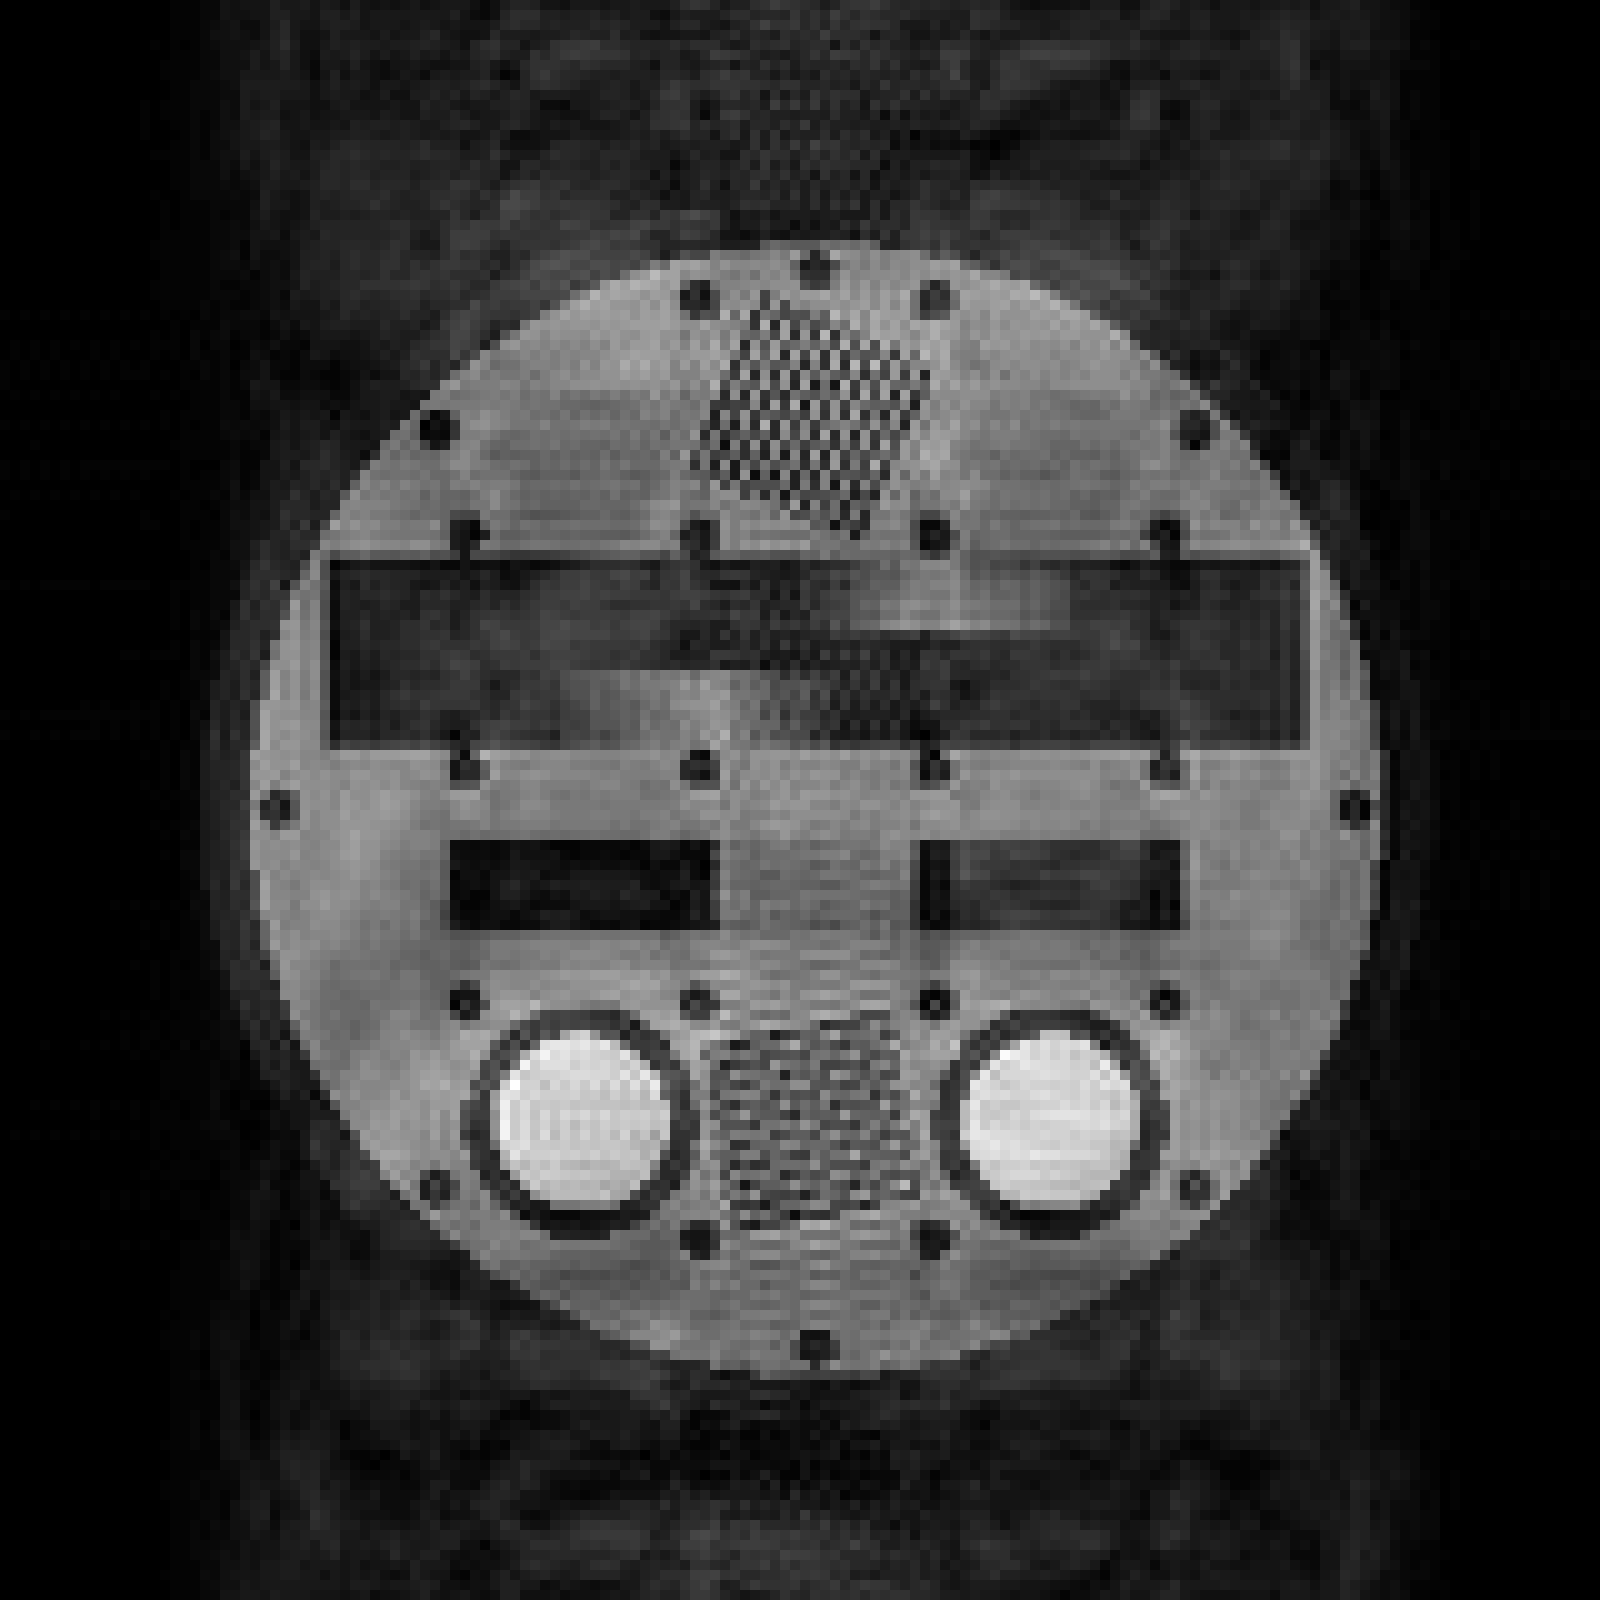
\includegraphics[width=0.47\textwidth]{img/results/lmk/EPI/Series25_OUT.png}}
	\
	\subcaptionbox{Differenzbild $D[i,j]$}{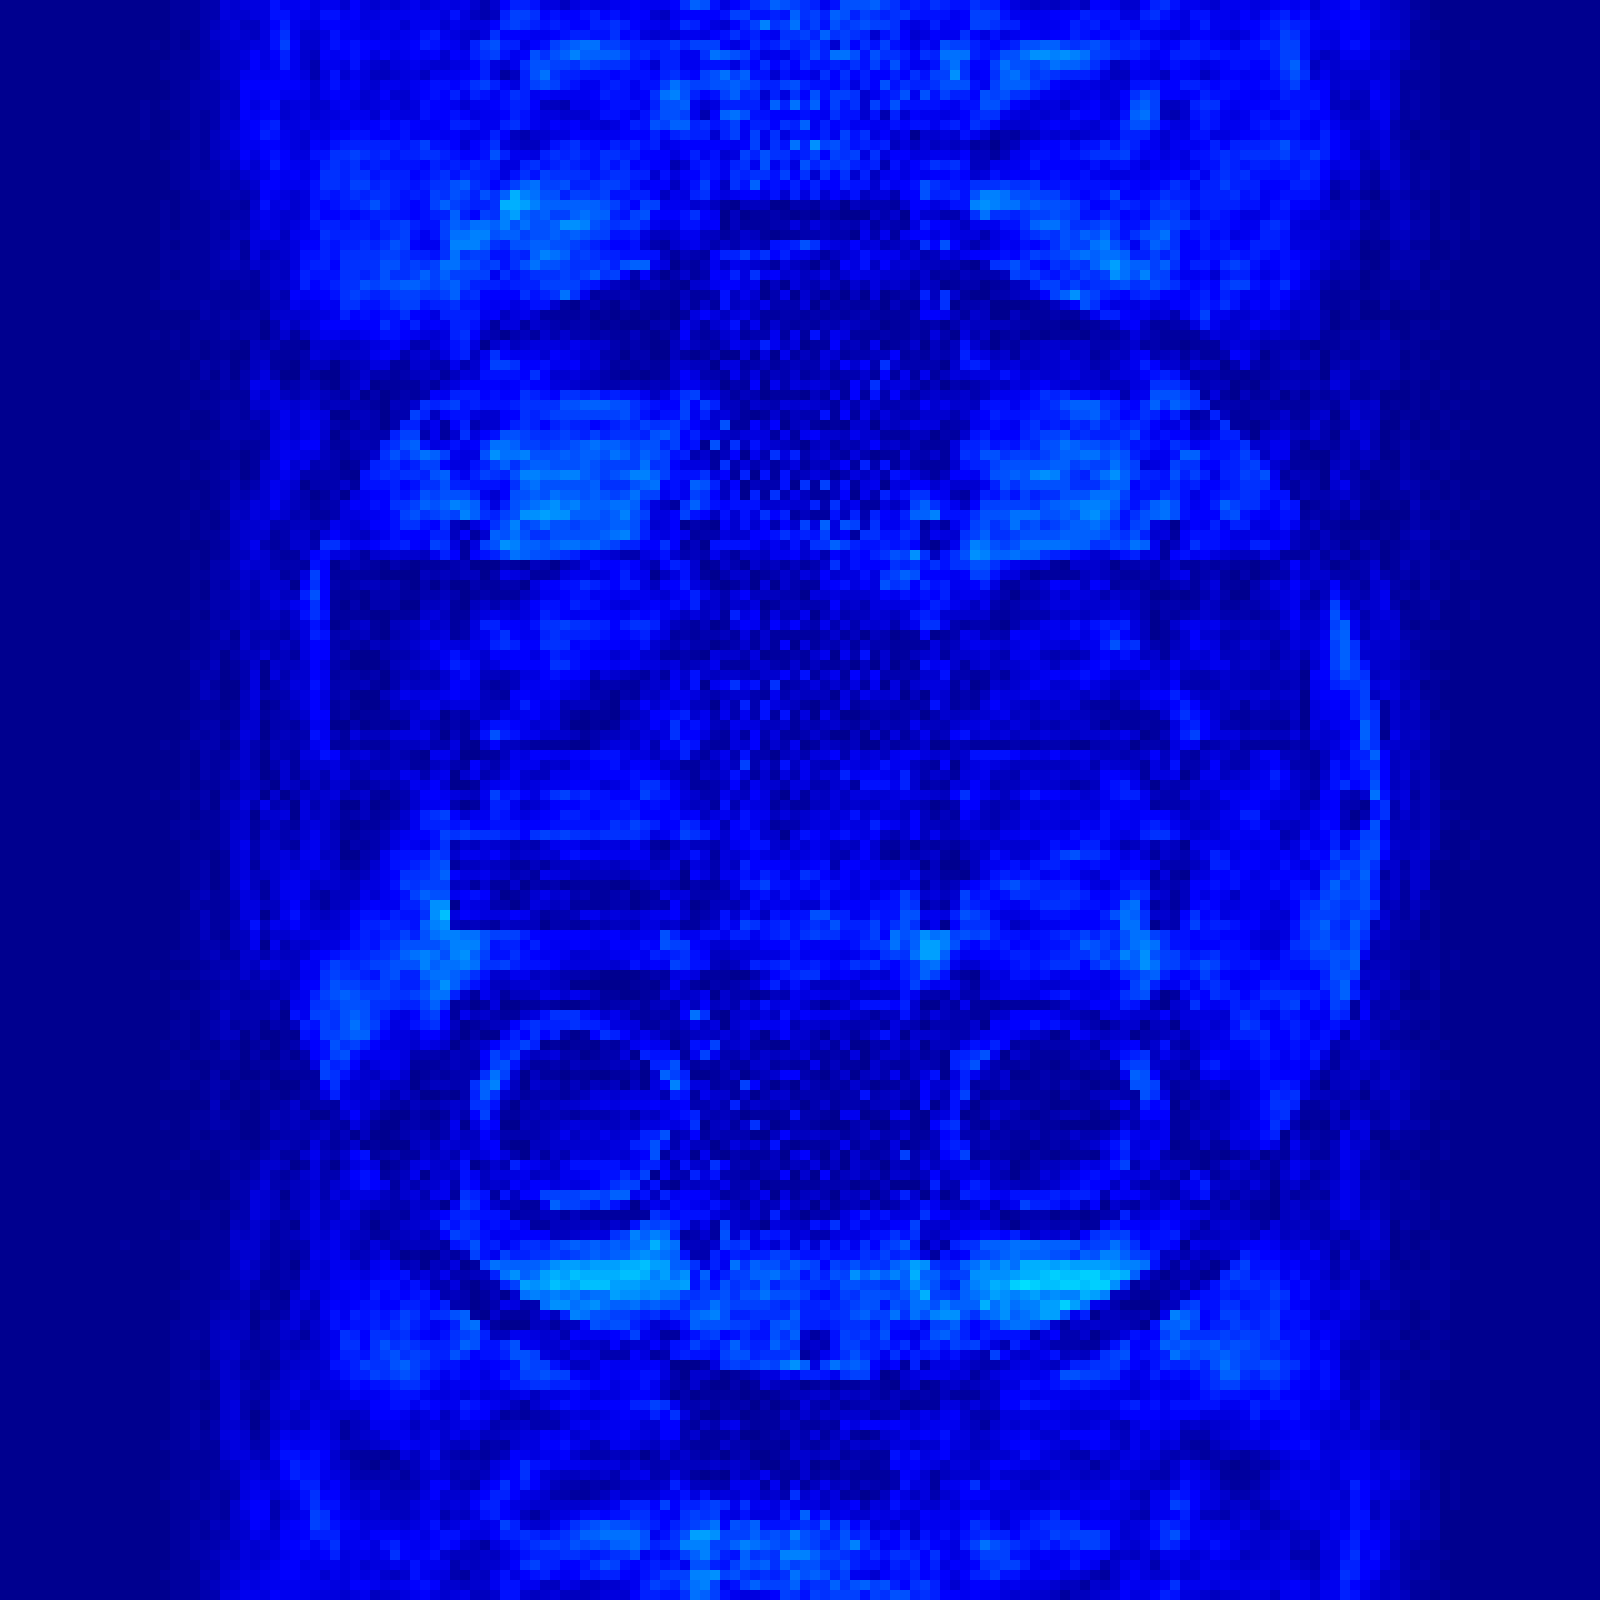
\includegraphics[width=0.47\textwidth]{img/results/lmk/EPI/Series25_DIFF.png}}
	\caption[LMK04821 in MR-Tomograph mit aktivem Gradientensystem (EPI) (3)]{Simulationsergebnis LMK04821 in MR-Tomograph mit aktivem Gradientensystem (EPI-Sequenz); $MSE=0.0085$, $SSIM=0.6552$}
	\label{fig:resLMKepi3}	
\end{figure}






\section{($1/f$)-Phasenrauschen}

\subsection{Spinecho-Sequenz}

\begin{figure}[H]
	\centering
	\subcaptionbox{Rekonstruiertes Schnittbild}{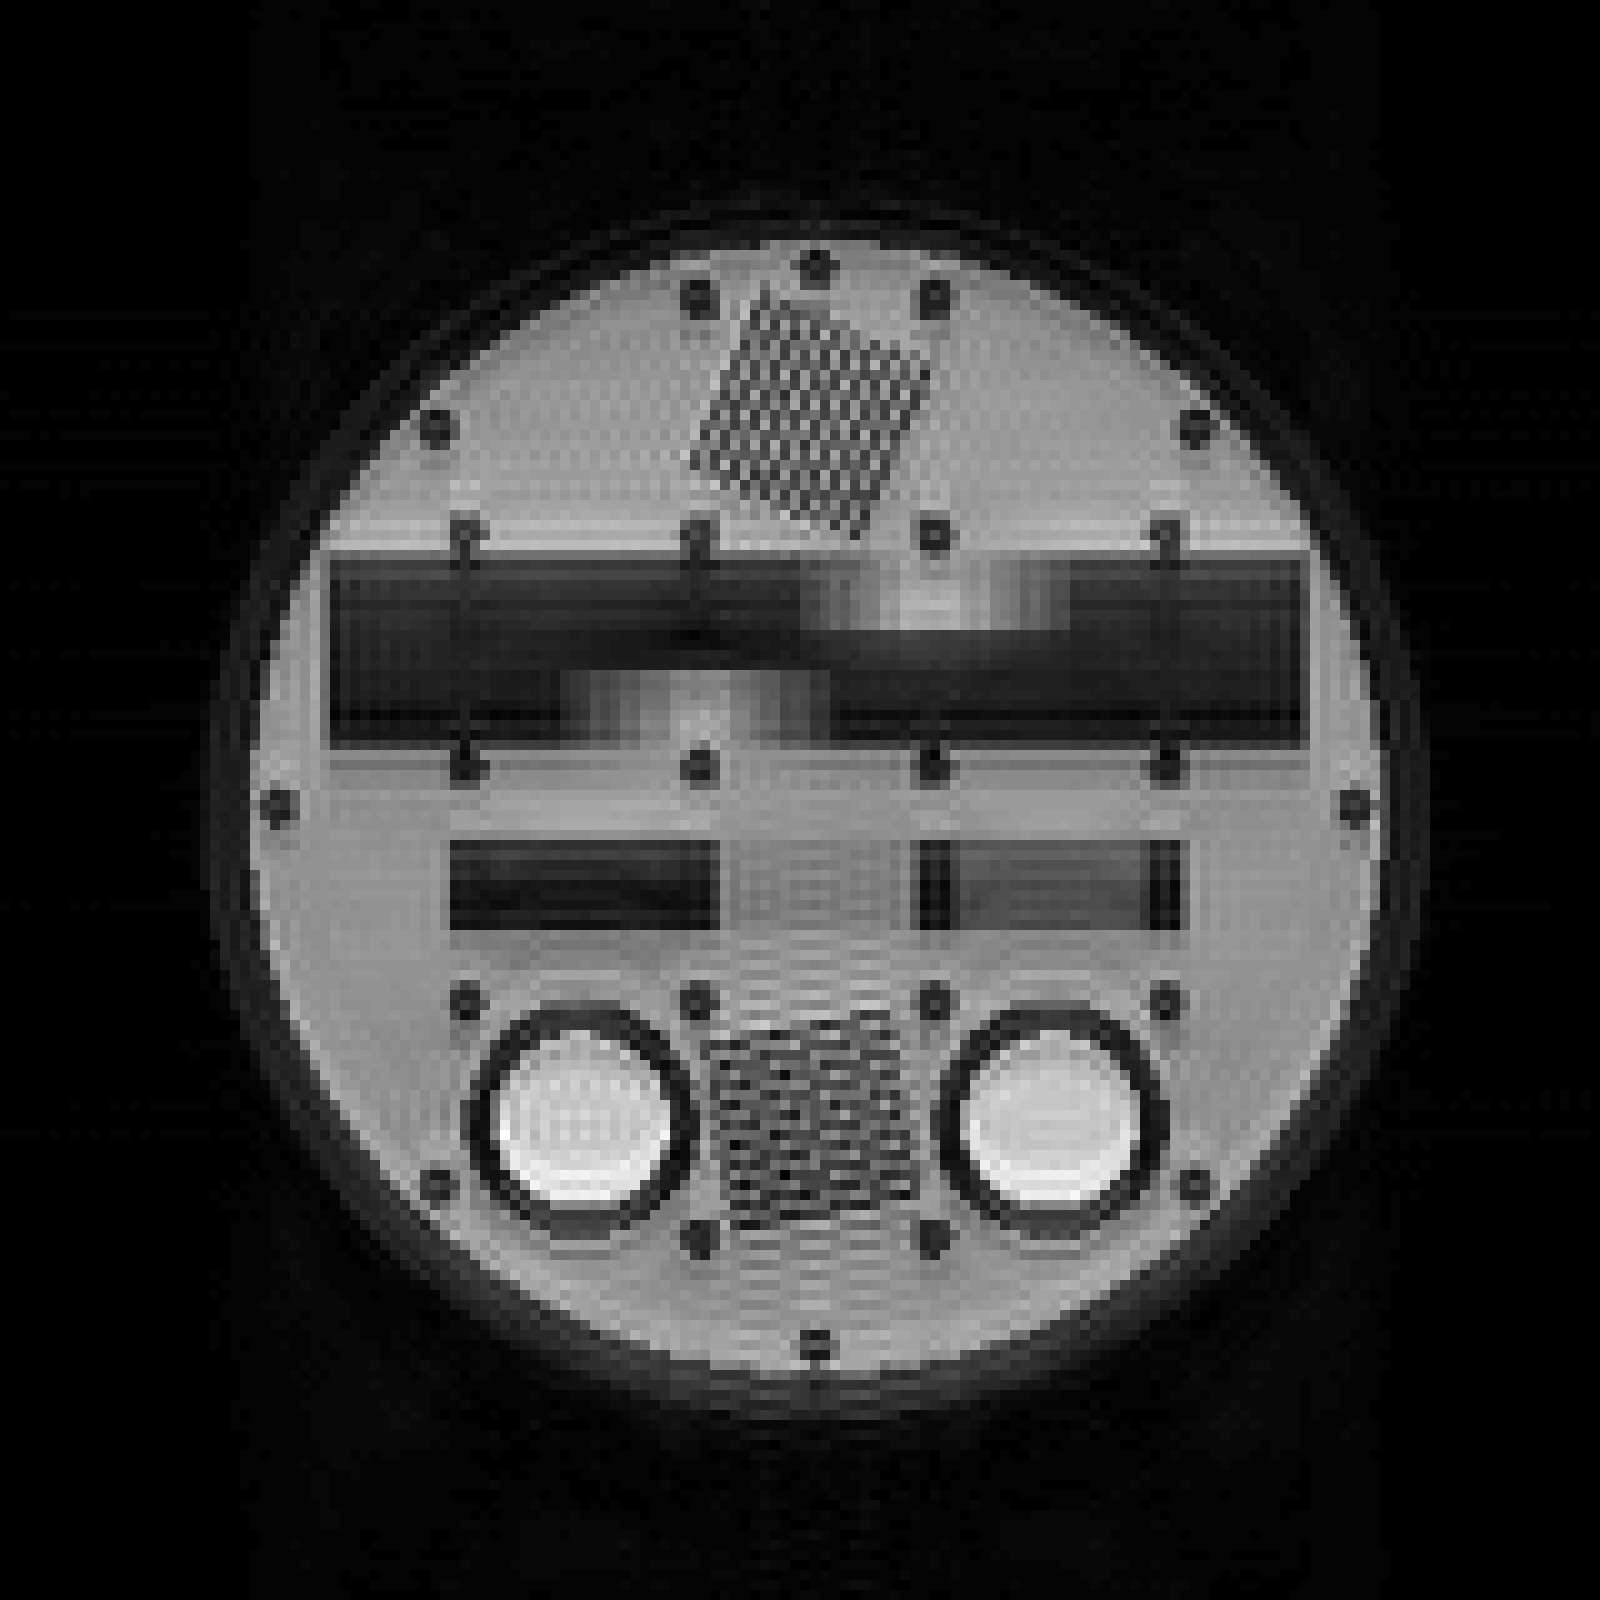
\includegraphics[width=0.47\textwidth]{img/results/cumsum/SE/Series21_OUT.png}}
	\
	\subcaptionbox{Differenzbild $D[i,j]$}{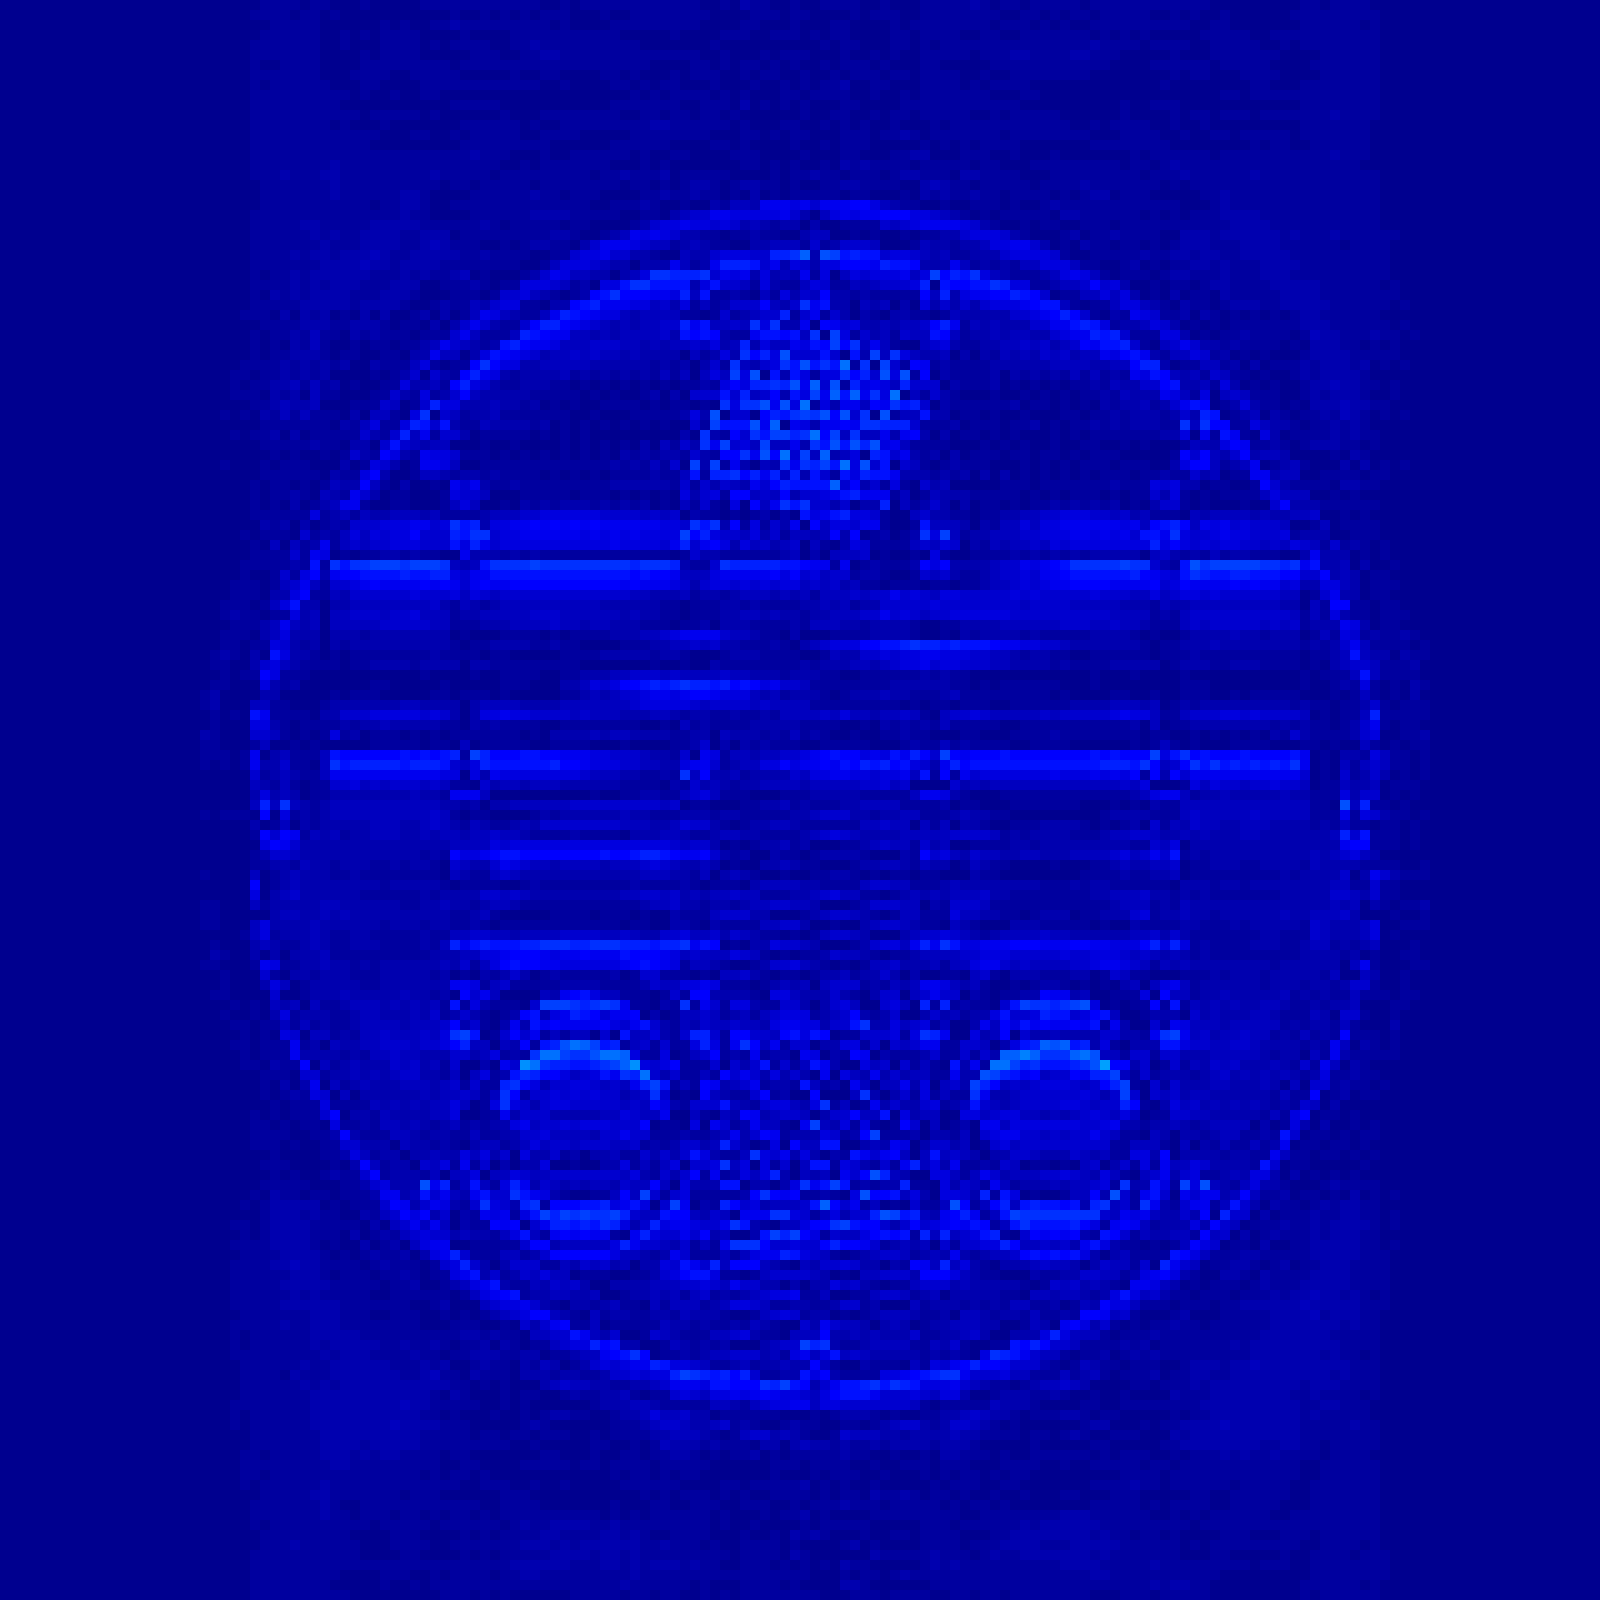
\includegraphics[width=0.47\textwidth]{img/results/cumsum/SE/Series21_DIFF.png}}
	\caption[Simulationsergebnis reines $1/f$-Phasenrauschen (SE) (1)]{Simulationsergebnis reines $1/f$-Phasenrauschen (Spinecho-Sequenz); $MSE=0.0019$, $SSIM=0.8335$}
	\label{fig:res1overFse1}	
\end{figure}

\begin{figure}[H]
	\centering
	\subcaptionbox{Rekonstruiertes Schnittbild}{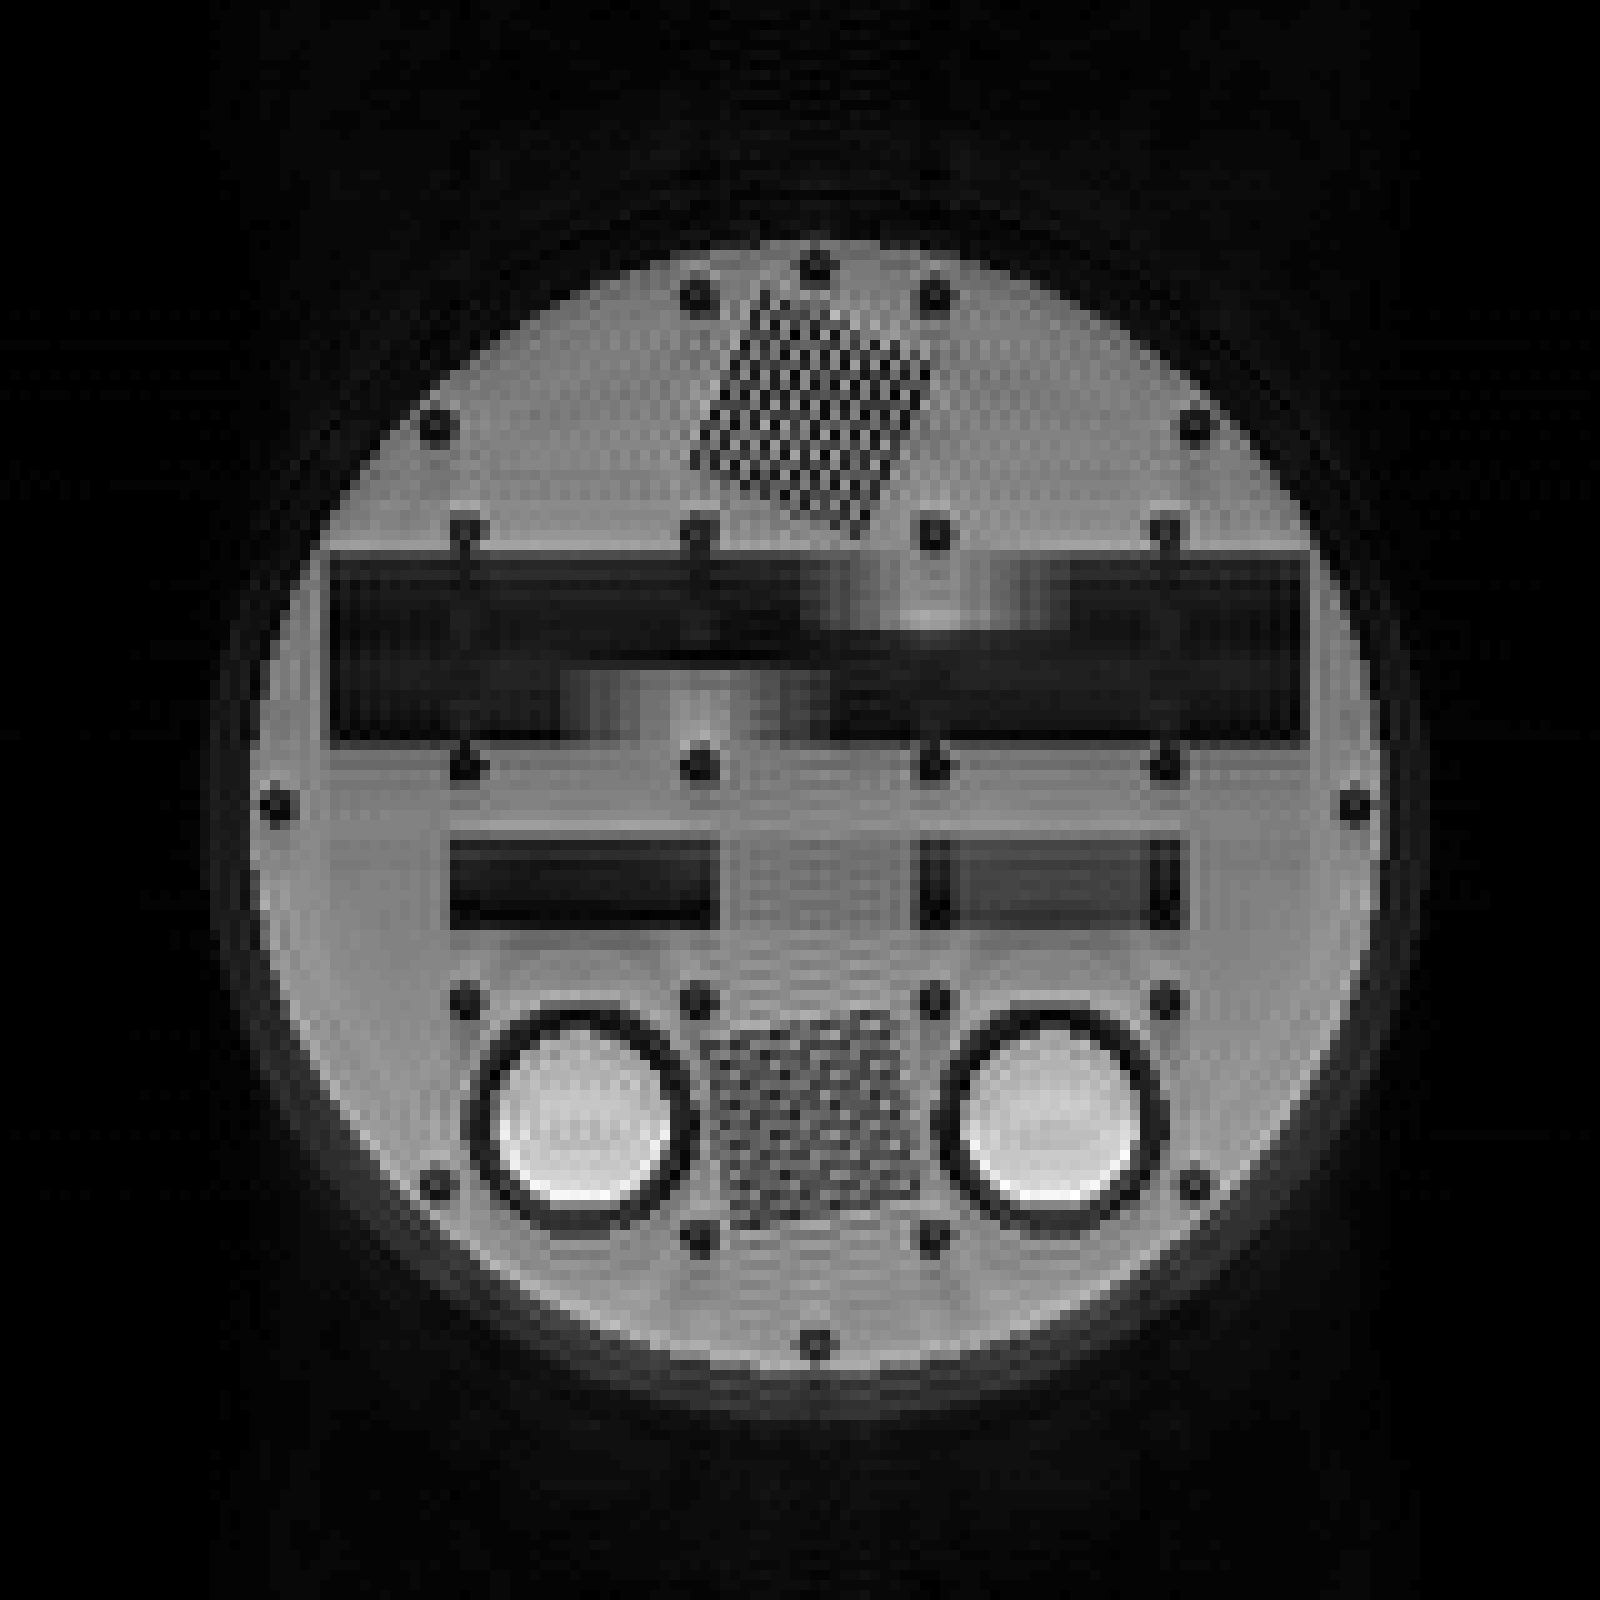
\includegraphics[width=0.47\textwidth]{img/results/cumsum/SE/Series22_OUT.png}}
	\
	\subcaptionbox{Differenzbild $D[i,j]$}{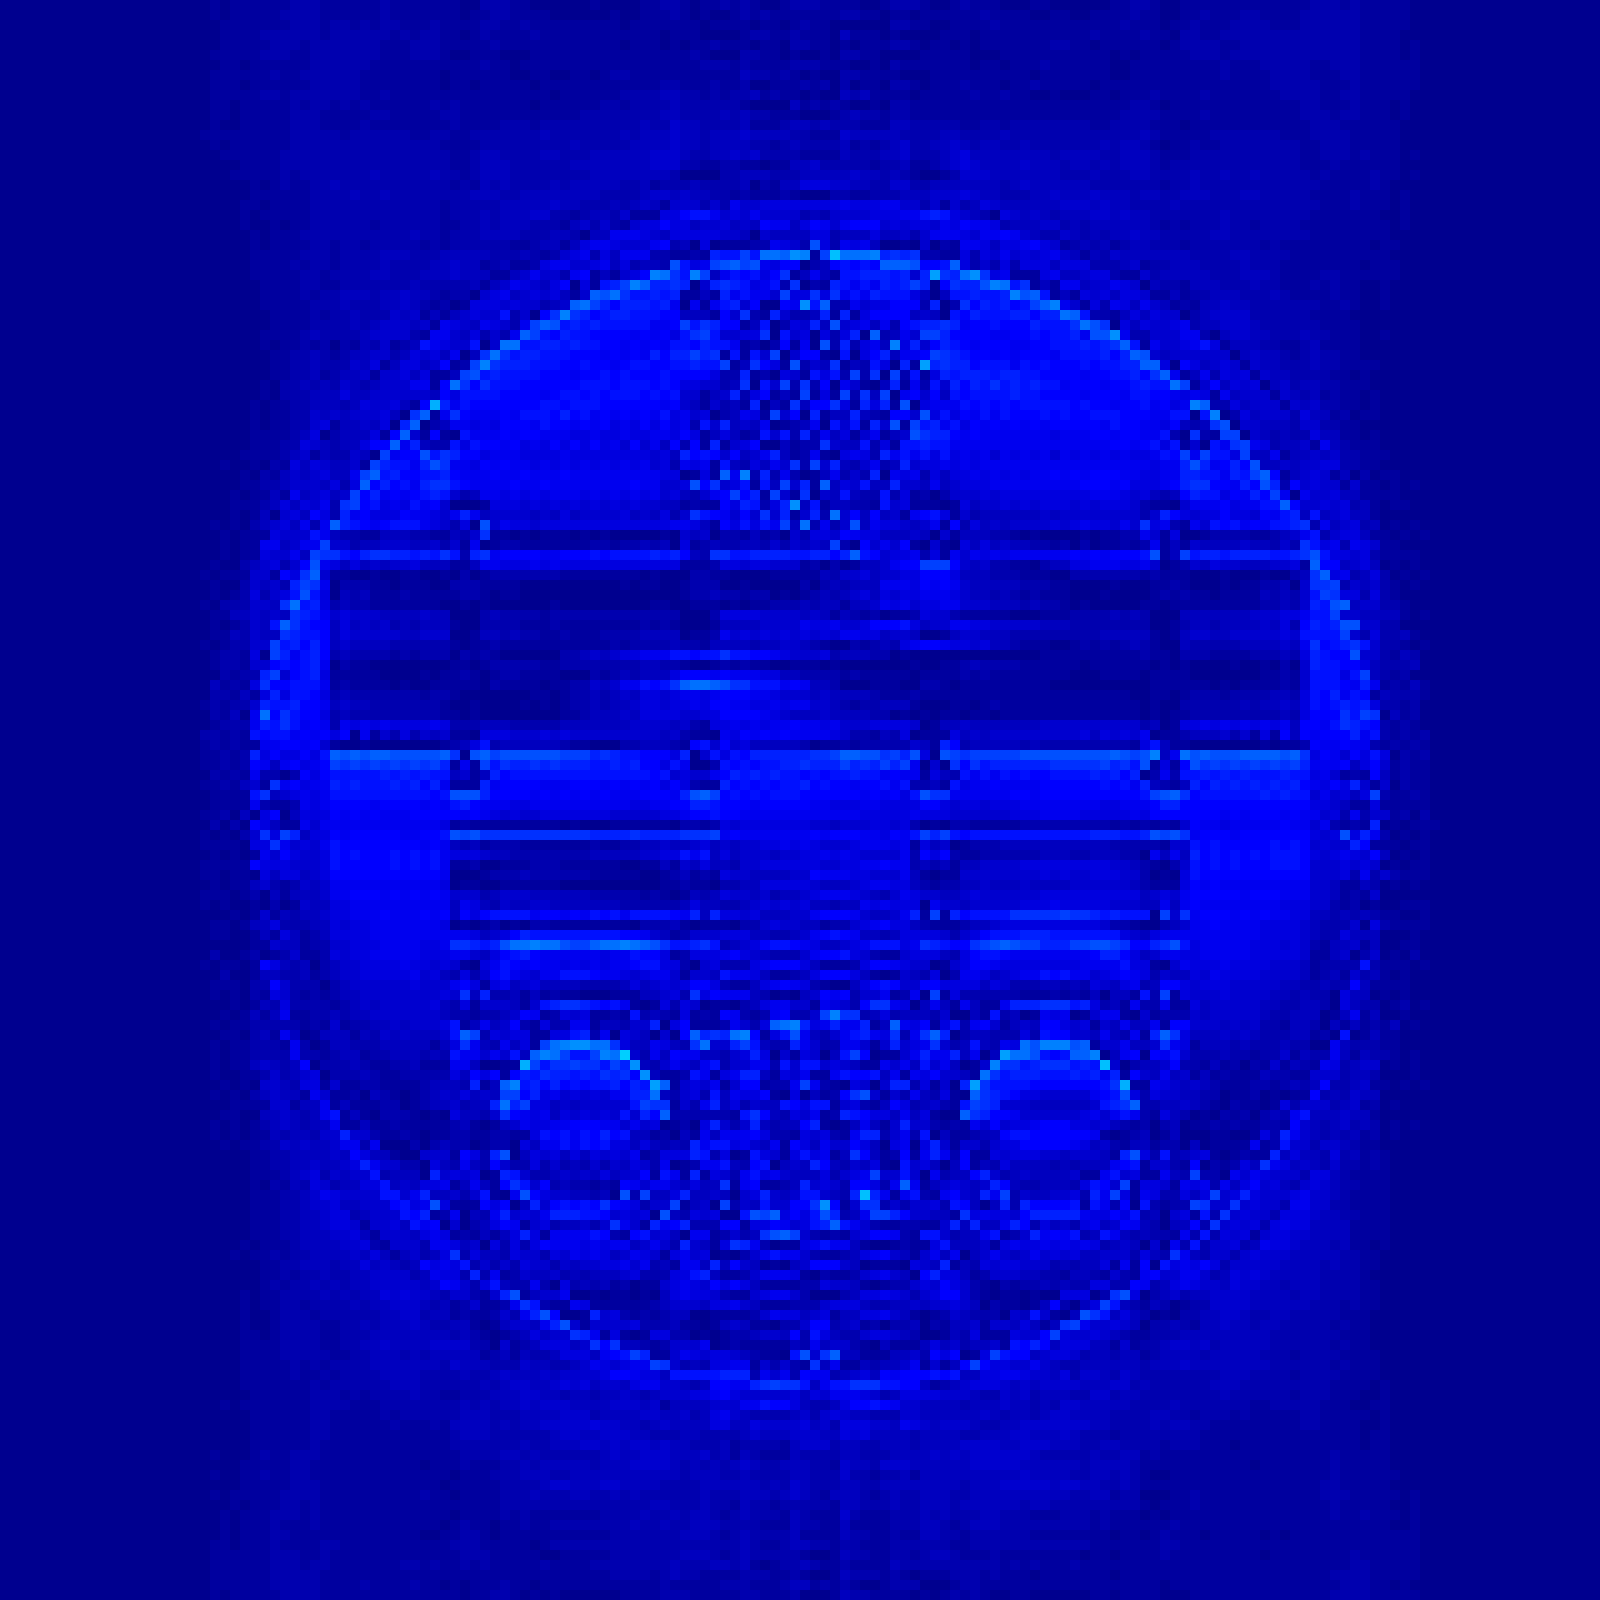
\includegraphics[width=0.47\textwidth]{img/results/cumsum/SE/Series22_DIFF.png}}
	\caption[Simulationsergebnis reines $1/f$-Phasenrauschen (SE) (2)]{Simulationsergebnis reines $1/f$-Phasenrauschen (Spinecho-Sequenz); $MSE=0.0037$, $SSIM=0.7465$}
	\label{fig:res1overFse2}	
\end{figure}

\begin{figure}[H]
	\centering
	\subcaptionbox{Rekonstruiertes Schnittbild}{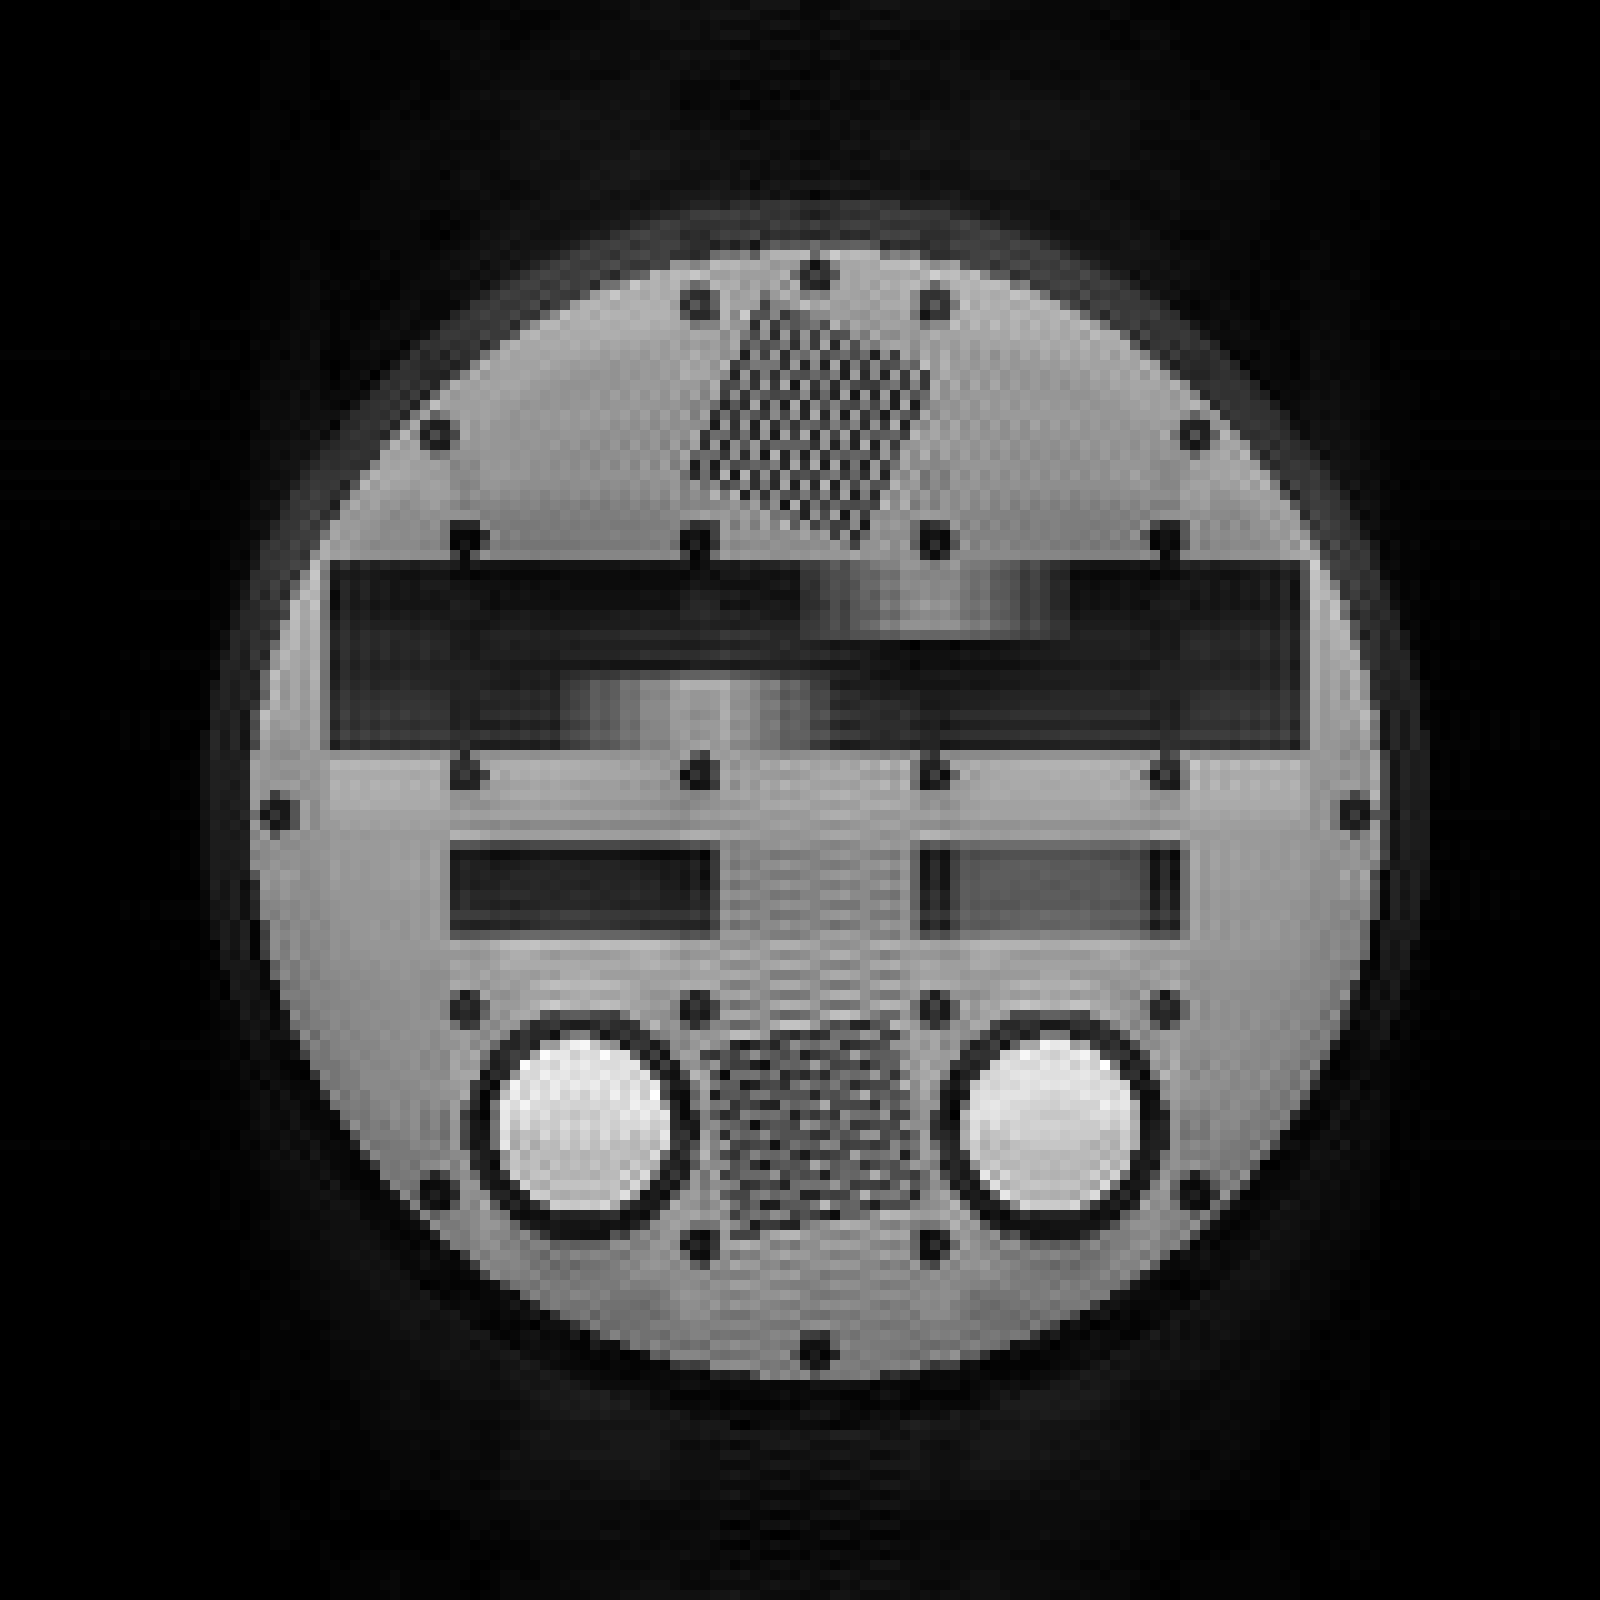
\includegraphics[width=0.47\textwidth]{img/results/cumsum/SE/Series23_OUT.png}}
	\
	\subcaptionbox{Differenzbild $D[i,j]$}{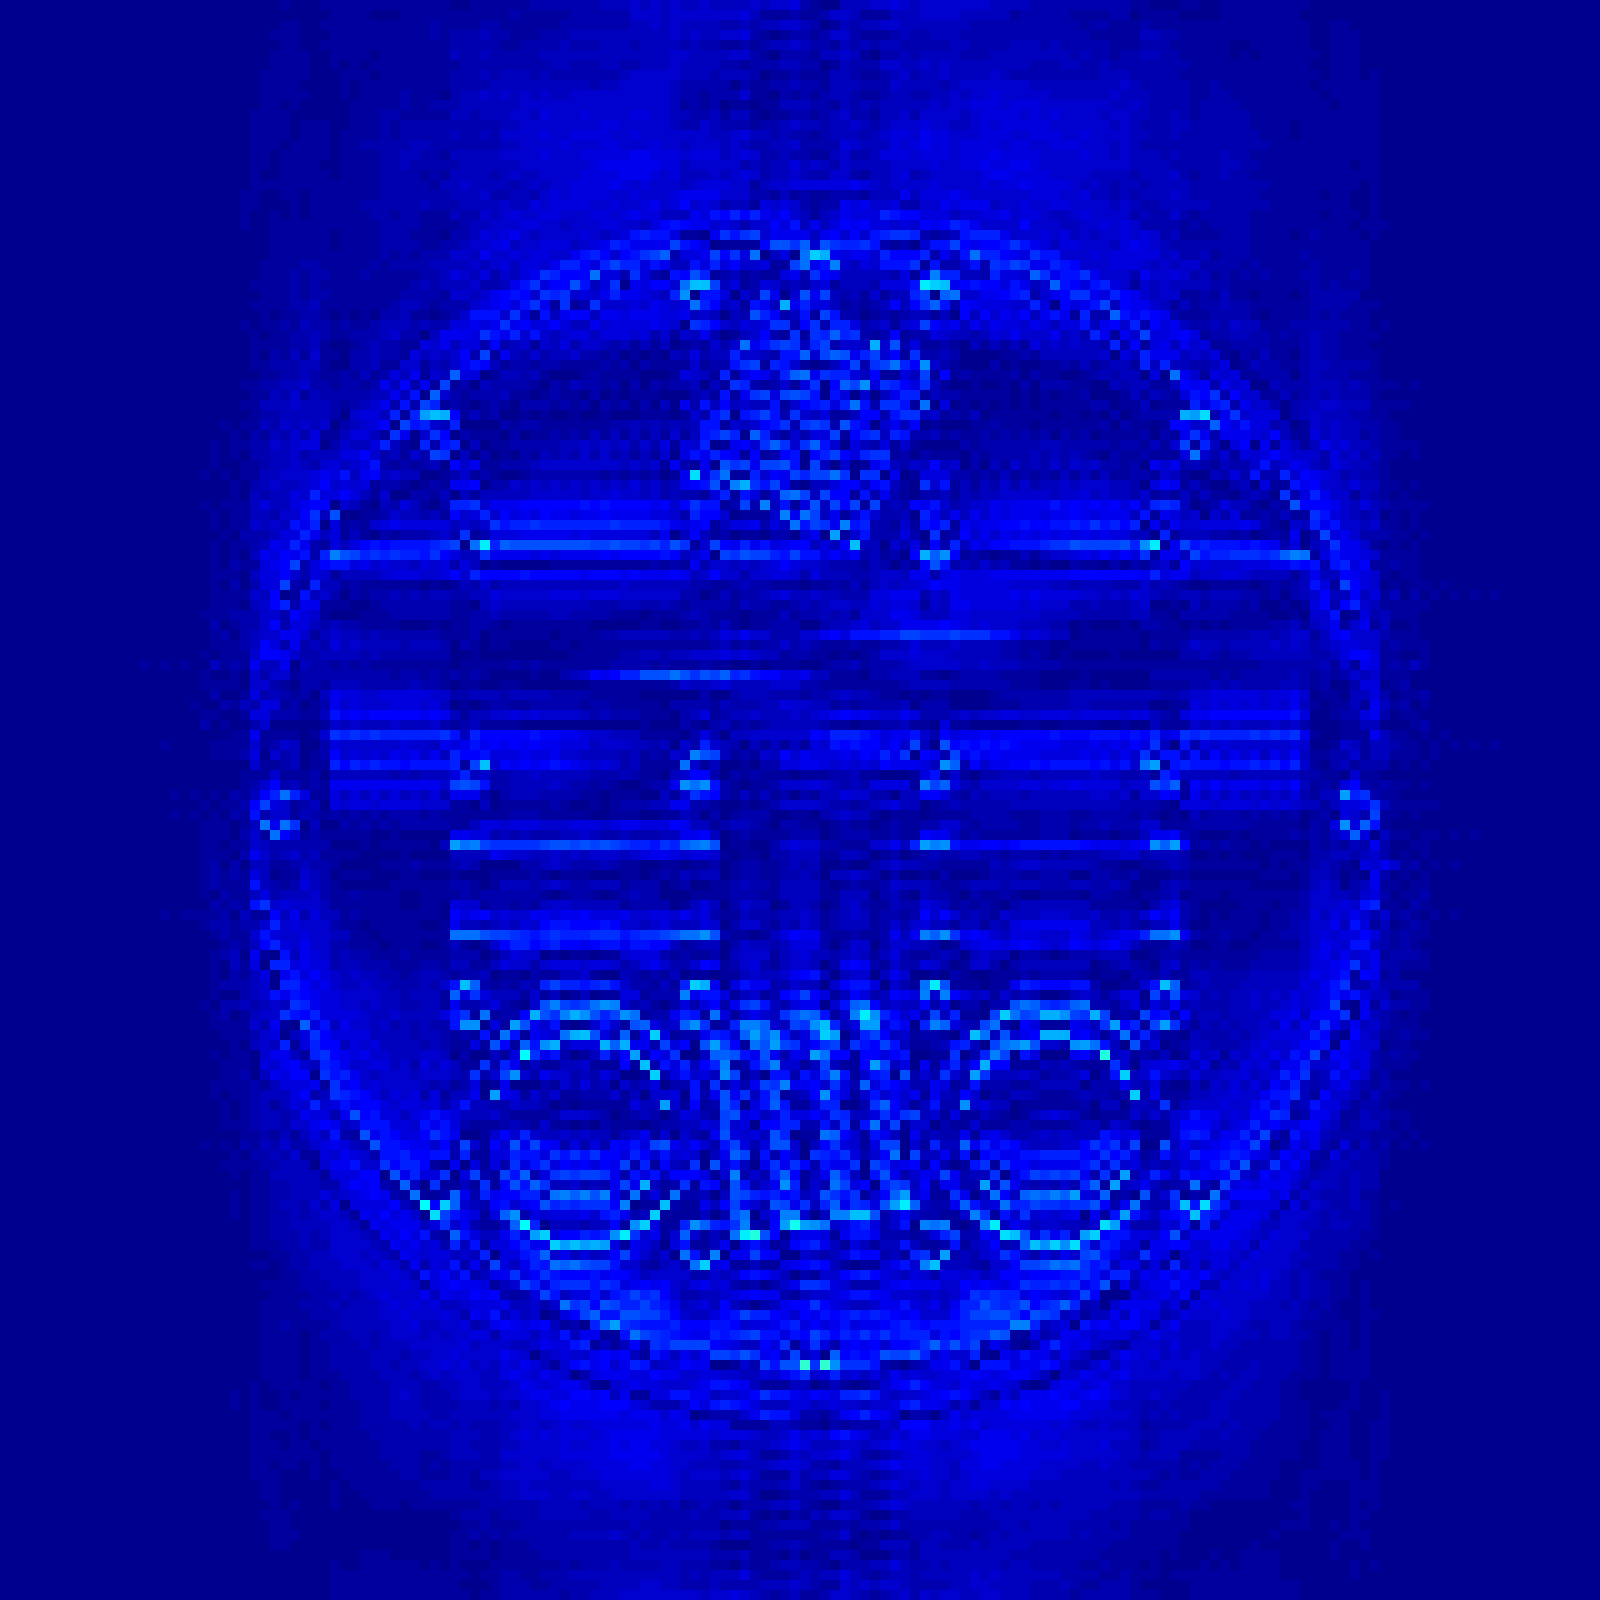
\includegraphics[width=0.47\textwidth]{img/results/cumsum/SE/Series23_DIFF.png}}
	\caption[Simulationsergebnis reines $1/f$-Phasenrauschen (SE) (3)]{Simulationsergebnis reines $1/f$-Phasenrauschen (Spinecho-Sequenz); $MSE=0.0041$, $SSIM=0.7079$}
	\label{fig:res1overFse3}	
\end{figure}

\subsection{EPI-Sequenz}

\begin{figure}[H]
	\centering
	\subcaptionbox{Rekonstruiertes Schnittbild}{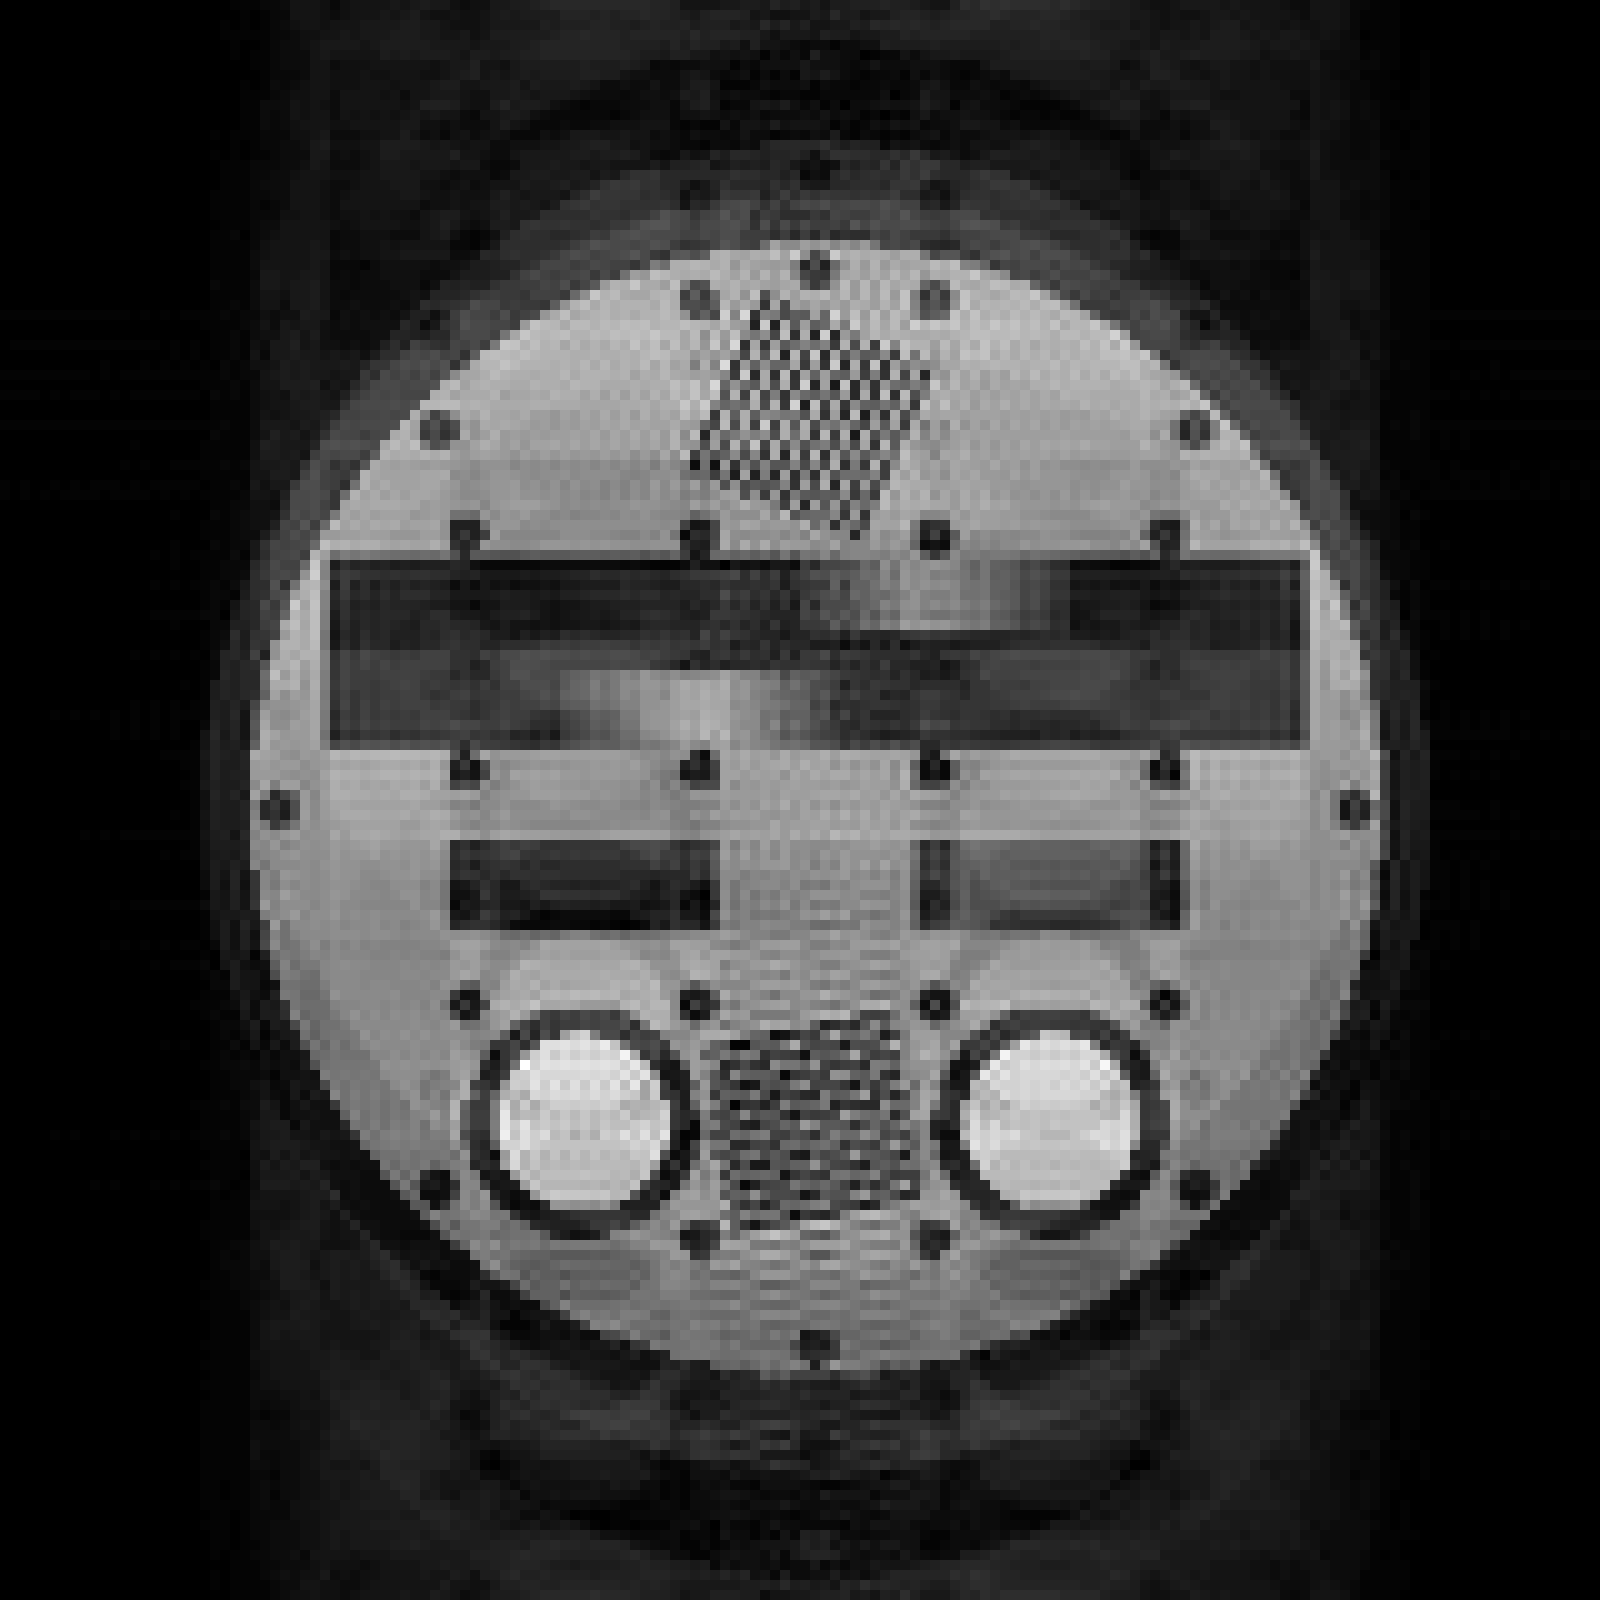
\includegraphics[width=0.47\textwidth]{img/results/cumsum/EPI/Series26_OUT.png}}
	\
	\subcaptionbox{Differenzbild $D[i,j]$}{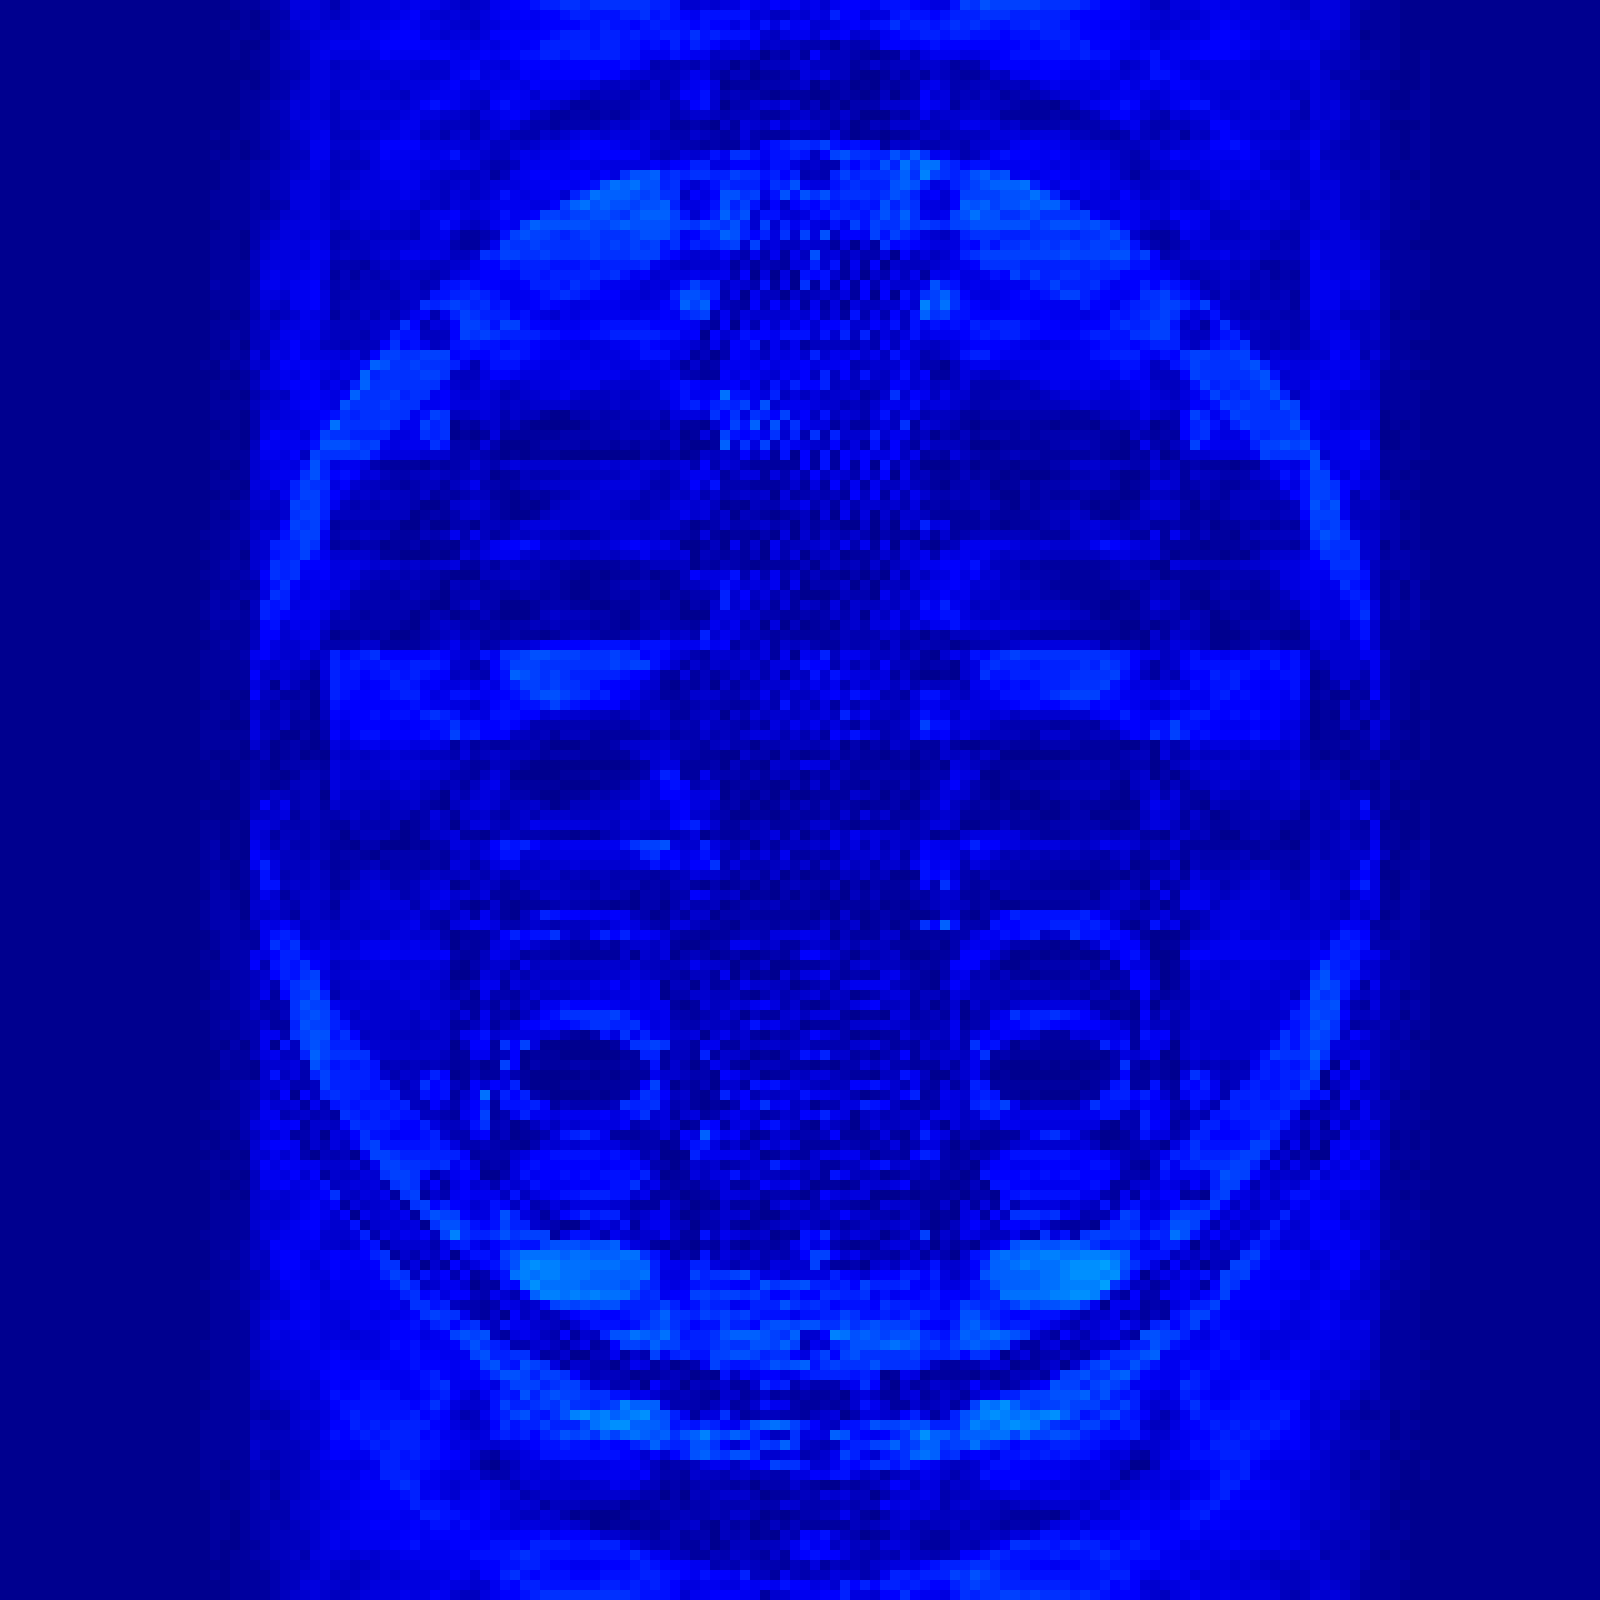
\includegraphics[width=0.47\textwidth]{img/results/cumsum/EPI/Series26_DIFF.png}}
	\caption[Simulationsergebnis reines $1/f$-Phasenrauschen (EPI) (1)]{Simulationsergebnis reines $1/f$-Phasenrauschen (EPI-Sequenz); $MSE=0.0060$, $SSIM=0.6875$}
	\label{fig:res1overFepi1}	
\end{figure}

\begin{figure}[H]
	\centering
	\subcaptionbox{Rekonstruiertes Schnittbild}{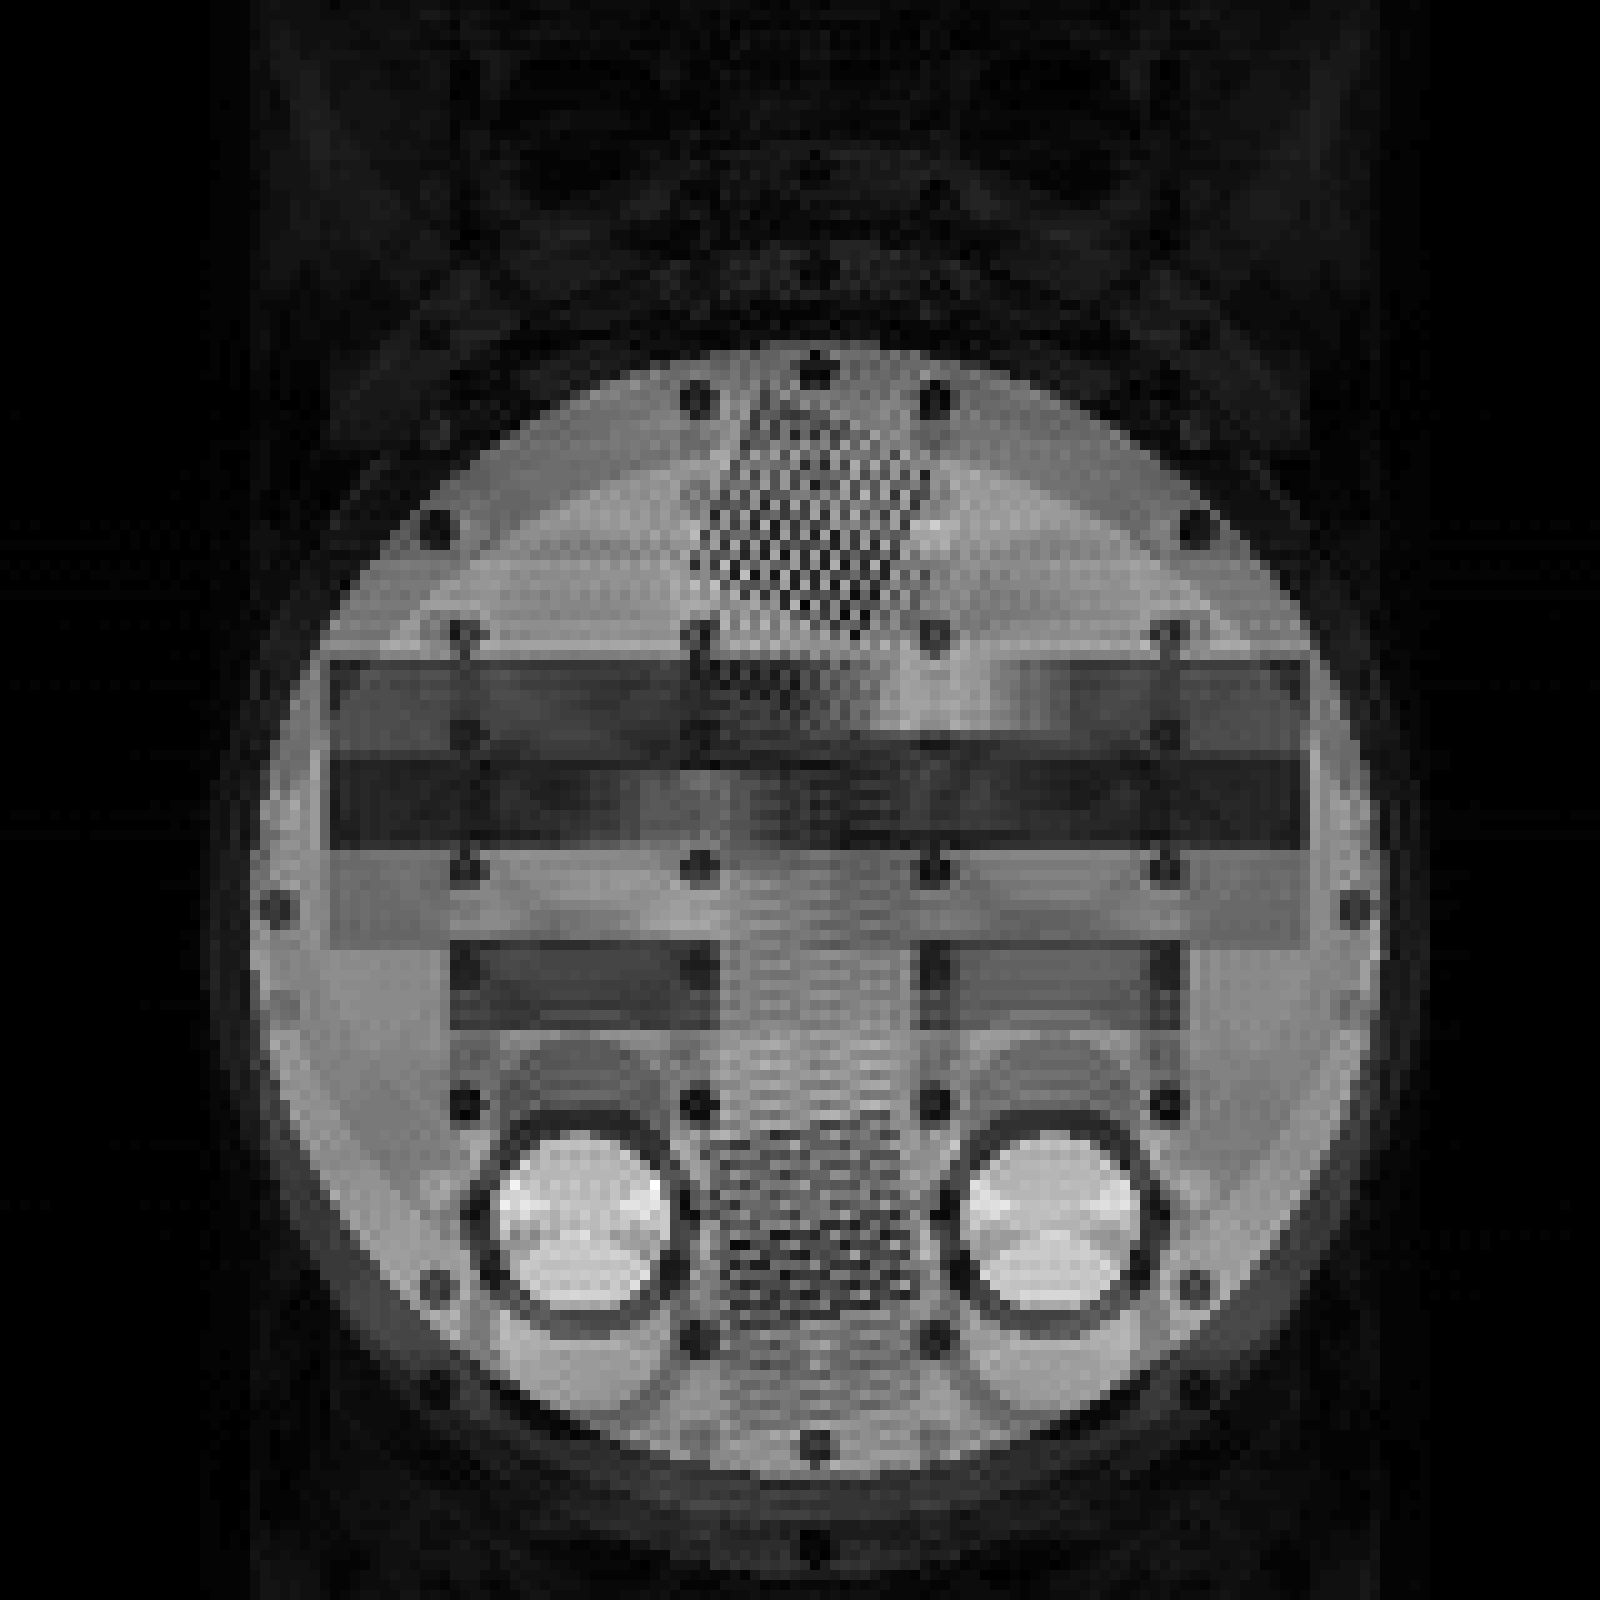
\includegraphics[width=0.47\textwidth]{img/results/cumsum/EPI/Series28_OUT.png}}
	\
	\subcaptionbox{Differenzbild $D[i,j]$}{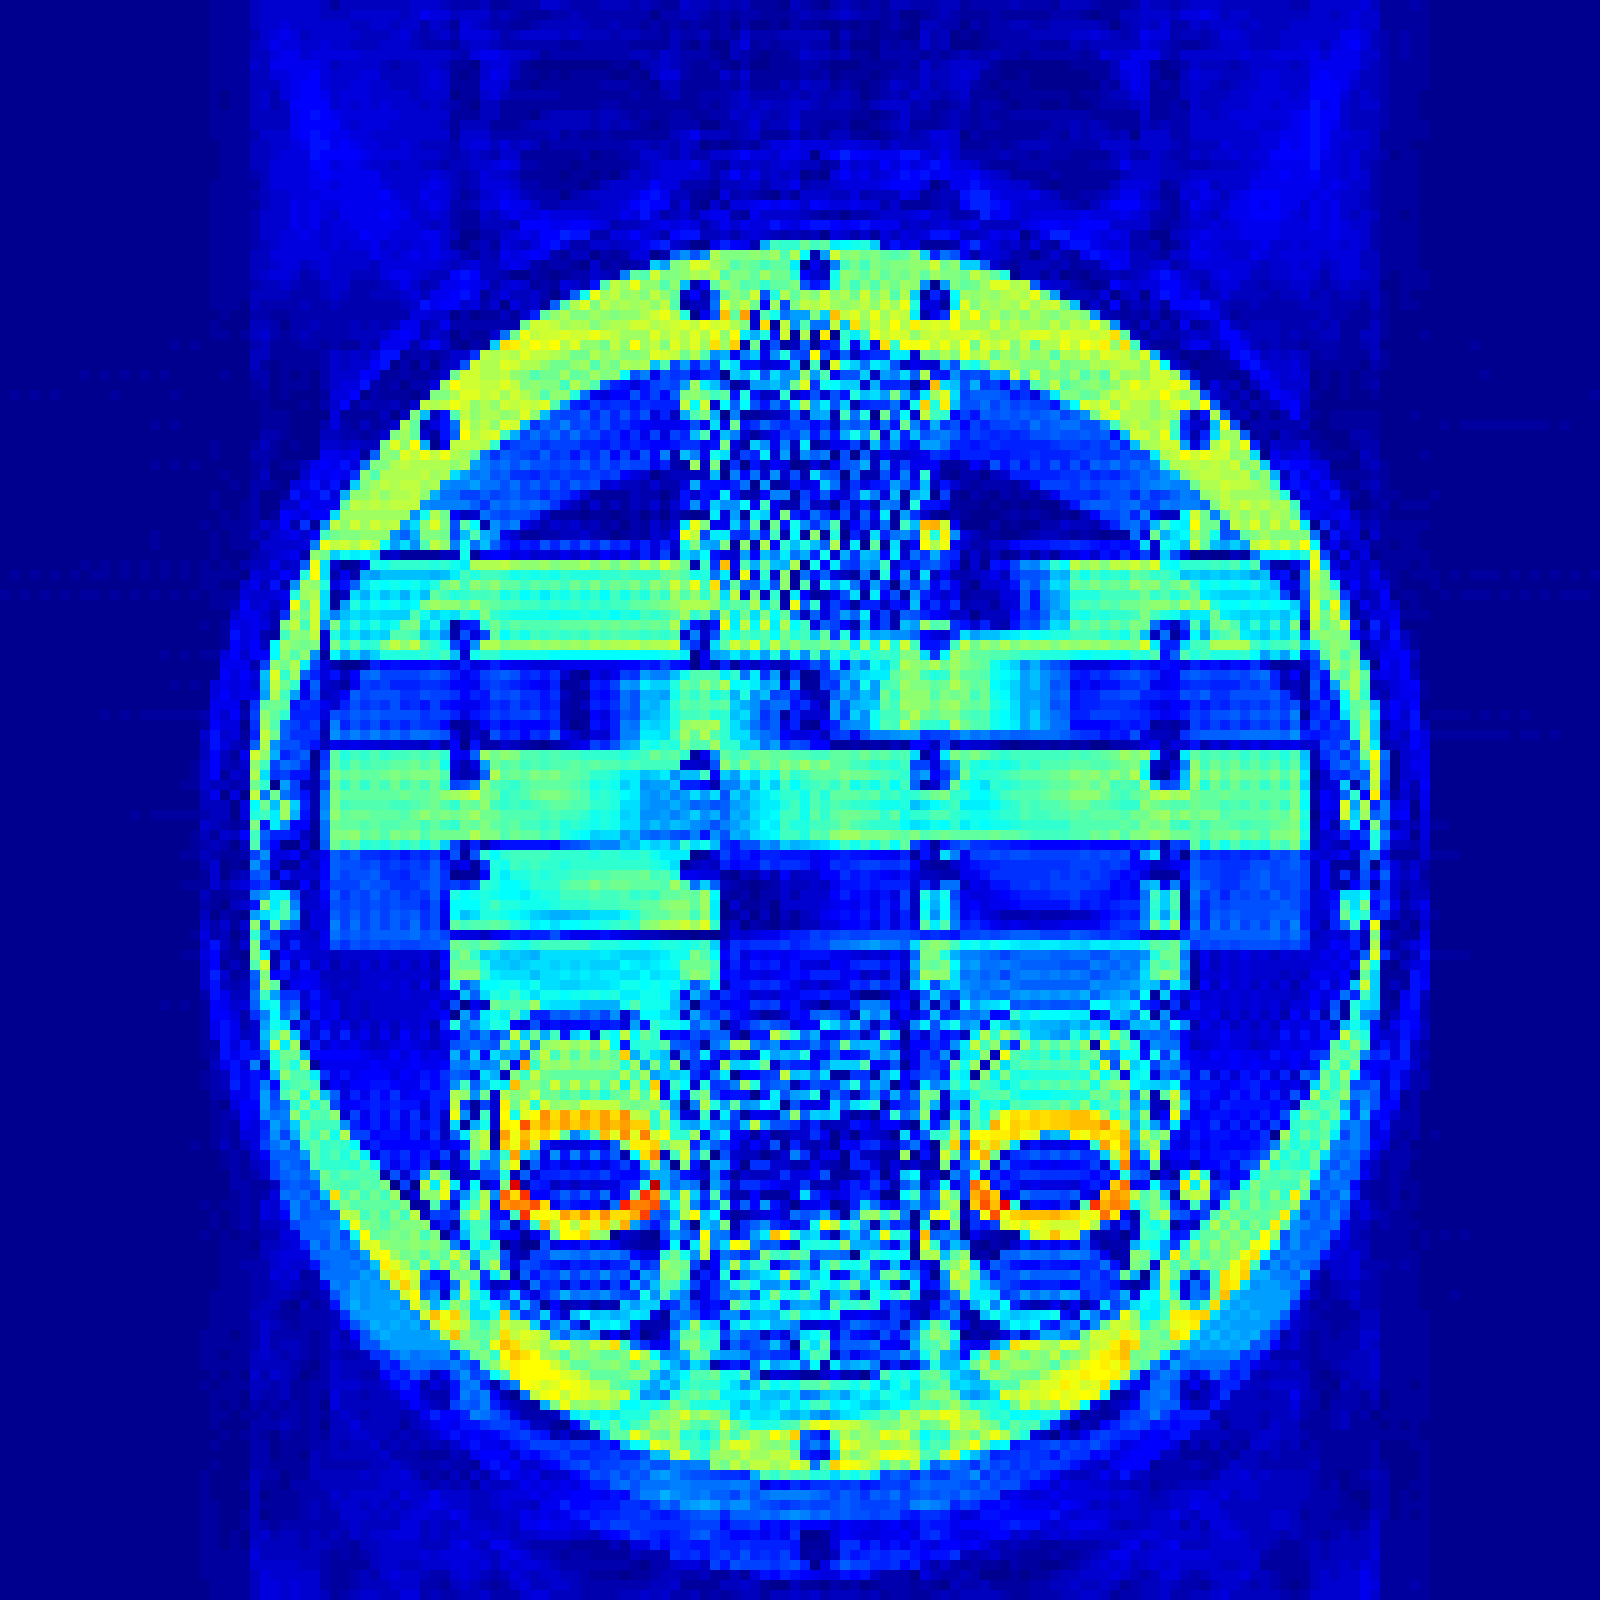
\includegraphics[width=0.47\textwidth]{img/results/cumsum/EPI/Series28_DIFF.png}}
	\caption[Simulationsergebnis reines $1/f$-Phasenrauschen (EPI) (2)]{Simulationsergebnis reines $1/f$-Phasenrauschen (EPI-Sequenz); $MSE=0.0541$, $SSIM=0.4756$}
	\label{fig:res1overFepi2}	
\end{figure}

\begin{figure}[H]
	\centering
	\subcaptionbox{Rekonstruiertes Schnittbild}{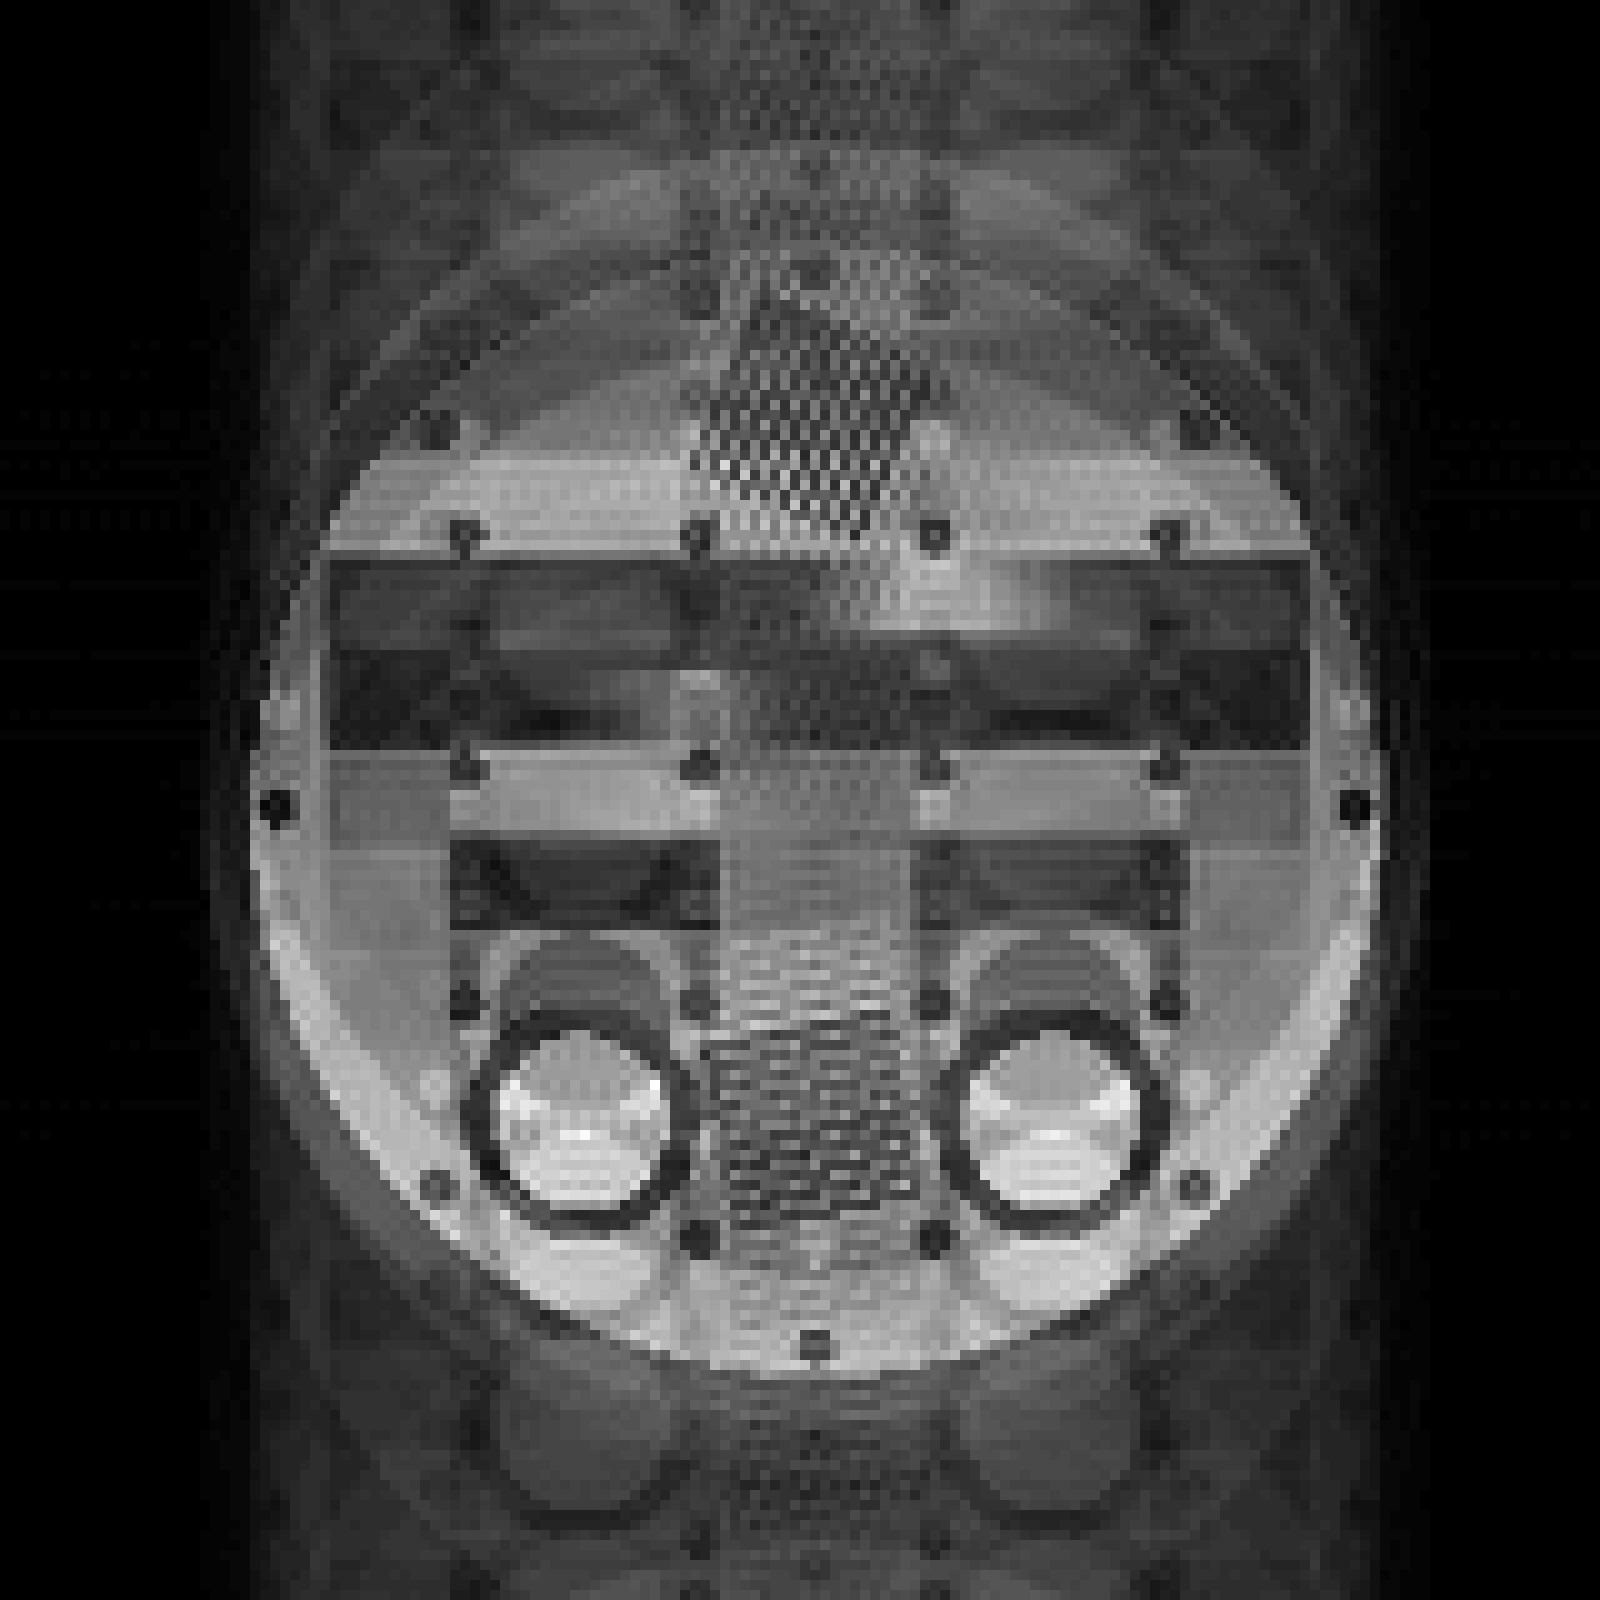
\includegraphics[width=0.47\textwidth]{img/results/cumsum/EPI/Series30_OUT.png}}
	\
	\subcaptionbox{Differenzbild $D[i,j]$}{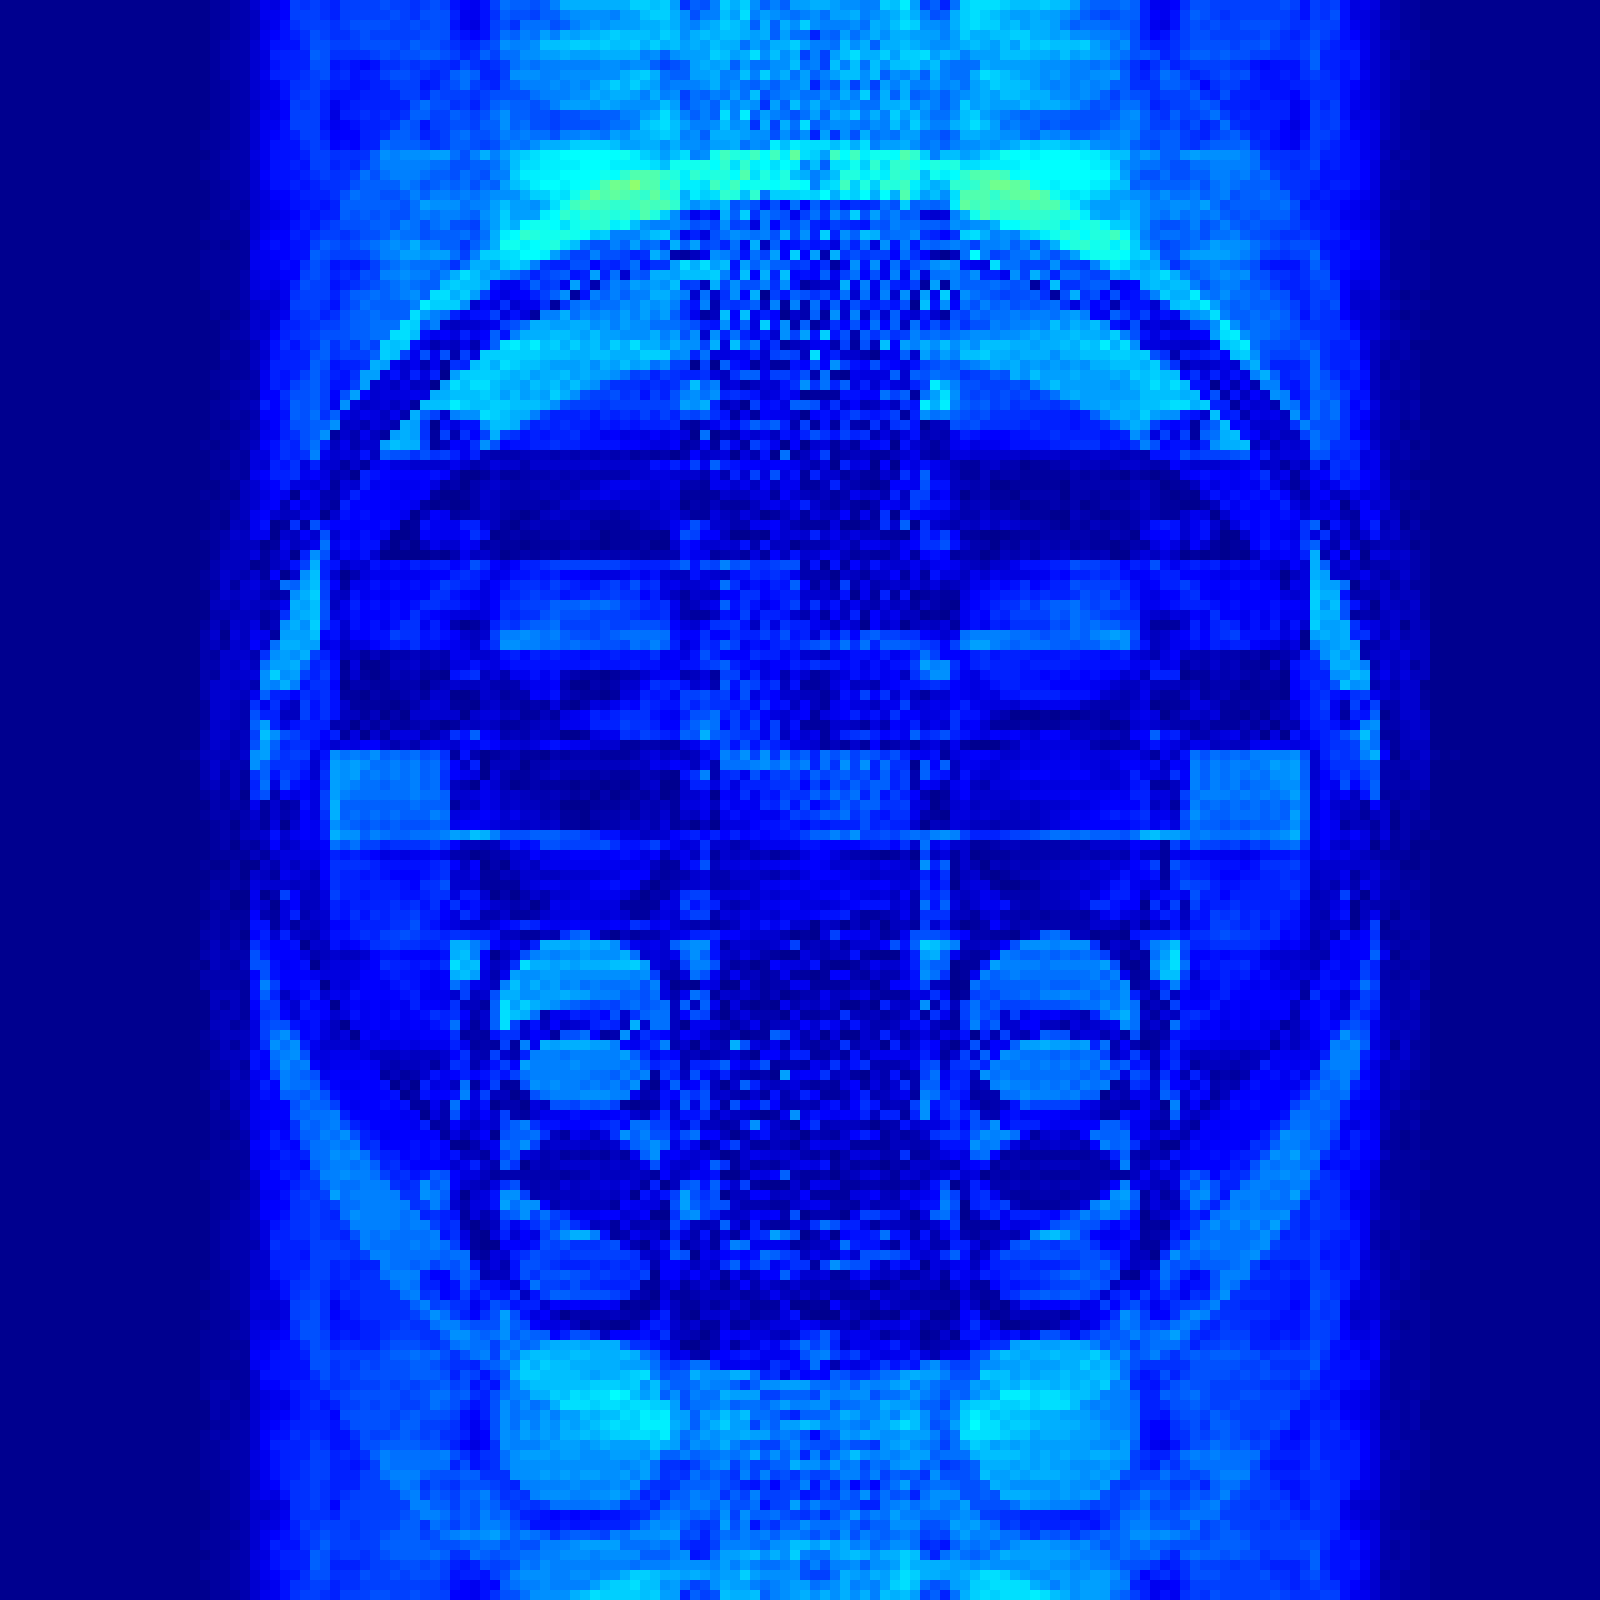
\includegraphics[width=0.47\textwidth]{img/results/cumsum/EPI/Series30_DIFF.png}}
	\caption[Simulationsergebnis reines $1/f$-Phasenrauschen (EPI) (3)]{Simulationsergebnis reines $1/f$-Phasenrauschen (EPI-Sequenz); $MSE=0.0220$, $SSIM=0.6010$}
	\label{fig:res1overFepi3}	
\end{figure}

\section{Diskussion der Ergebnisse}

















